% ============================================================
%  Chapter 6 — Experiment 1: Multimodal Bot Detection
%  Include with: % ============================================================
%  Chapter 6 — Experiment 1: Multimodal Bot Detection
%  Include with: % ============================================================
%  Chapter 6 — Experiment 1: Multimodal Bot Detection
%  Include with: % ============================================================
%  Chapter 6 — Experiment 1: Multimodal Bot Detection
%  Include with: \include{bot-detection/chapter6_experiment1}
%  Figures are referenced relative to the dissertation root.
% ============================================================

\chapter{Experiment 1: Multimodal Bot Detection with a Bidirectional LSTM}
\label{chap:experiment1}

Chapter~5 closed with a note about evaluation methodology that shapes
everything in this chapter: accuracy figures commonly reported for bot
detection systems are often products of dataset construction artefacts
rather than genuine generalisation capability. Keeping that in mind, this
chapter does not aim to set a benchmark record. It aims to build a working
detection system that uses both structured account metadata and unstructured
tweet text, understand what the model has learned from each source, and
report its performance honestly against published baselines.

The model chosen is a Bidirectional Long Short-Term Memory network with a
self-attention mechanism and a sentence-embedding text branch. It is trained
on the Cresci-2017 corpus, which provides labelled account metadata and tweet
content for over thirteen thousand Twitter accounts.

% ----------------------------------------------------------------
\section{Experimental Objectives}
% ----------------------------------------------------------------

The experiment has three concrete goals. The first is to construct a feature
representation that is suitable for sequential processing from two
heterogeneous sources: tabular account metadata and raw tweet text. The second
is to train a bidirectional recurrent model that fuses both sources and record
its behaviour across training epochs in enough detail to reason about
convergence and the contribution of each branch. The third is to situate the
result within the published literature with a clear account of why direct
comparisons are more complicated than a single table of numbers suggests.

A wider aim underlies these goals. The trained model will serve as the
baseline detector in Experiment~2, where it will be tested against synthetic
bot accounts generated by a large language model. Its performance on that
adversarial task is arguably more informative about its practical utility than
its performance on held-out data from the same distribution, and the two
chapters should be read together with that in mind.

% ----------------------------------------------------------------
\section{Dataset: Cresci-2017}
\label{sec:cresci}
% ----------------------------------------------------------------

Several publicly available datasets were considered for this experiment.
TwiBot-22 is the largest and most recent~\cite{AZS+23}, but it requires a
formal access request and its network-graph structure would push the
experiment toward a graph neural network architecture. TwiBot-20 is open but
still large, with over 229,000 accounts and 33 million tweets. Cresci-2017
was selected because it is open, well-documented, widely used as a
benchmark, and contains both account metadata and tweet content in a single
download. It is also the dataset for which the evaluation problems discussed
in Section~5.7 have been most carefully studied~\cite{HSR+23}, which means
the limitations can be stated precisely.

\subsection{Composition}

The corpus was collected from Twitter and assembled by Cresci and colleagues
as part of a study on second-generation social spambots. It contains genuine
accounts whose human authorship was verified by the original authors, and
several categories of automated accounts spanning older spam bots, social
spambots of varying sophistication, and fake follower networks. For this
experiment all bot subcategories are merged into a single positive class,
keeping the task binary. The resulting dataset contains 13,240 accounts in
total, broken down by category in Table~\ref{tab:cresci_categories}.

\begin{table}[h]
\centering
\small
\caption{Composition of the Cresci-2017 dataset. All bot subcategories are
  treated as the positive class. Tweet availability indicates whether
  tweet content was present in the dataset download.}
\label{tab:cresci_categories}
\begin{tabular}{llrr}
\hline
\textbf{Category} & \textbf{Label} & \textbf{Accounts} & \textbf{Tweets} \\
\hline
Genuine accounts           & Human & 3{,}474 & 2{,}839{,}362 \\
Social spambots (type 1)   & Bot   &   991  & 1{,}610{,}034 \\
Social spambots (type 2)   & Bot   & 3{,}457 &   428{,}542 \\
Social spambots (type 3)   & Bot   &   464  & 1{,}418{,}557 \\
Traditional spambots       & Bot   & 1{,}000 &   145{,}094 \\
Fake followers             & Bot   & 3{,}351 &   196{,}027 \\
Other bot subcategories    & Bot   &   503  & none \\
\hline
\textbf{Total}             &       & \textbf{13{,}240} & \textbf{6{,}637{,}616} \\
\hline
\end{tabular}
\end{table}

The class imbalance is notable: bots outnumber humans by roughly 2.8 to 1.
Figure~\ref{fig:class_dist} shows this distribution visually. Of the 13,240
accounts, 10,197 have at least one tweet in the dataset and therefore receive
a non-zero text embedding. The remaining 3,043 accounts, concentrated in the
smaller bot subcategories that lack tweet data, contribute only their metadata
features to the model. Figure~\ref{fig:tweet_coverage} shows the breakdown by
category.

\begin{figure}[h]
  \centering
  \begin{minipage}{0.44\linewidth}
    \centering
    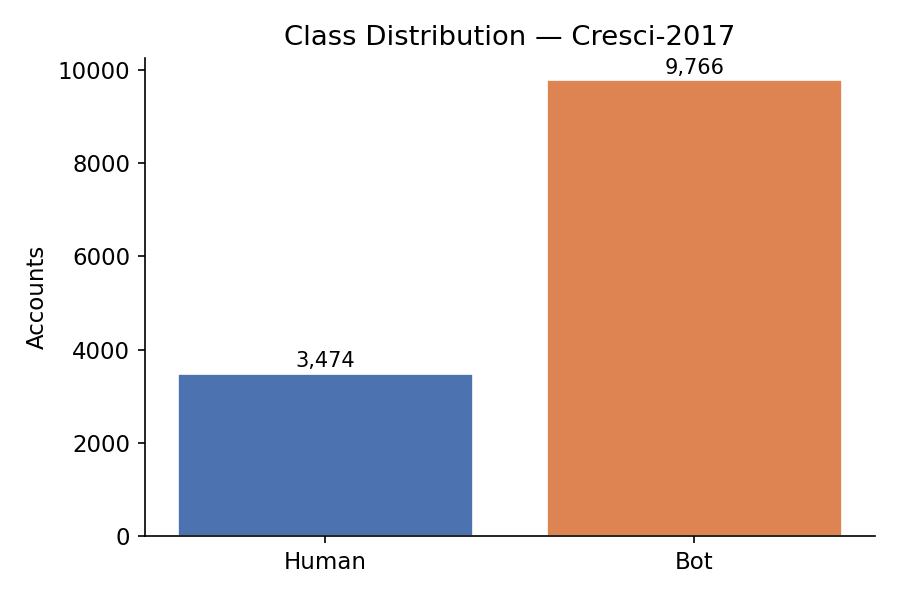
\includegraphics[width=\linewidth]{bot-detection/results/class_distribution.png}
    \caption{Class distribution of the Cresci-2017 dataset after merging all
      bot subcategories. The 2.8 to 1 imbalance is handled during training
      through weighted random sampling.}
    \label{fig:class_dist}
  \end{minipage}
  \hfill
  \begin{minipage}{0.52\linewidth}
    \centering
    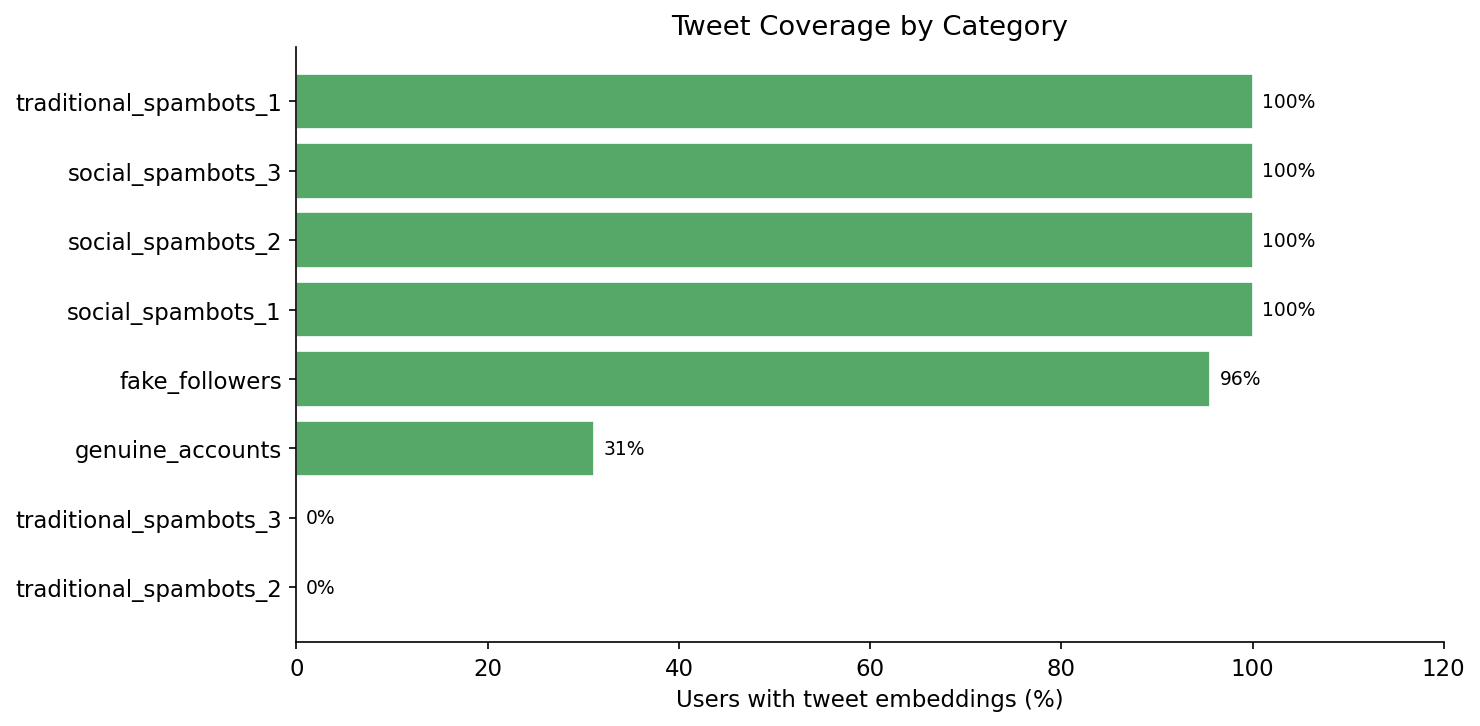
\includegraphics[width=\linewidth]{bot-detection/results/tweet_coverage.png}
    \caption{Proportion of accounts in each category that have tweet content
      available in the dataset. Categories without tweet data receive a zero
      embedding vector in the text branch.}
    \label{fig:tweet_coverage}
  \end{minipage}
\end{figure}

\subsection{Known Limitations}
\label{subsec:cresci_limits}

It would be dishonest to present this dataset without noting what
\citet{HSR+23} demonstrated about it. Bot accounts and human accounts in
Cresci-2017 were collected at different times through different pipelines,
which introduces a temporal correlation that has nothing to do with bot
behaviour. A simple decision tree trained only on account creation timestamps
achieves accuracy comparable to sophisticated models on this data, because
the creation dates of the two populations are systematically different. Any
model that includes creation-date derived features, as this one does through
account age, is implicitly exploiting that signal.

The performance figures reported later in this chapter show that the model
fits the dataset well. They do not show that it would generalise to a fresh
corpus of accounts collected under different conditions. Cross-dataset
evaluation would be the methodologically sound approach and is left to future
work given the scope of this thesis.

% ----------------------------------------------------------------
\section{Feature Engineering and Sequence Construction}
\label{sec:features}
% ----------------------------------------------------------------

The model takes two inputs per account: a structured metadata sequence and
a sentence embedding derived from the account's tweets. These are constructed
separately and fused inside the model.

\subsection{Metadata Features}

A standard LSTM expects a sequence of vectors as input, but account metadata
is a flat feature vector with no natural ordering. The solution adopted here
is to partition the features into four thematically coherent groups and treat
each group as one step in a four-step input sequence. The model then processes
these groups in both the forward and backward directions and learns which
combinations of behavioural dimensions are most diagnostic of automation.

The four groups are constructed as follows. The first covers network scale
and contains the log-transformed follower count, friend count, listed count,
and follower-to-friend ratio. The second covers activity scale and contains
log-transformed total statuses, total favourites, and per-day rates for both
posting and favouriting. The third covers profile flags and is the only binary
group, containing the four completeness and verification indicators. The fourth
covers derived ratios and contains log-transformed account age, a ratio of
total statuses to total favourites, a ratio of followers to listed count, and a
ratio of listed count to followers. Each group has exactly four features,
giving a metadata input tensor of shape $(N, 4, 4)$ for a batch of $N$
accounts. The three numeric groups are standardised with z-score normalisation
fitted on the training split; the binary group is left on its natural scale.

Figure~\ref{fig:feature_dist} shows the log-scale distributions of five
numeric features across both classes. The separation is already visible
without a classifier, particularly in posting rate and follower count.

\begin{figure}[h]
  \centering
  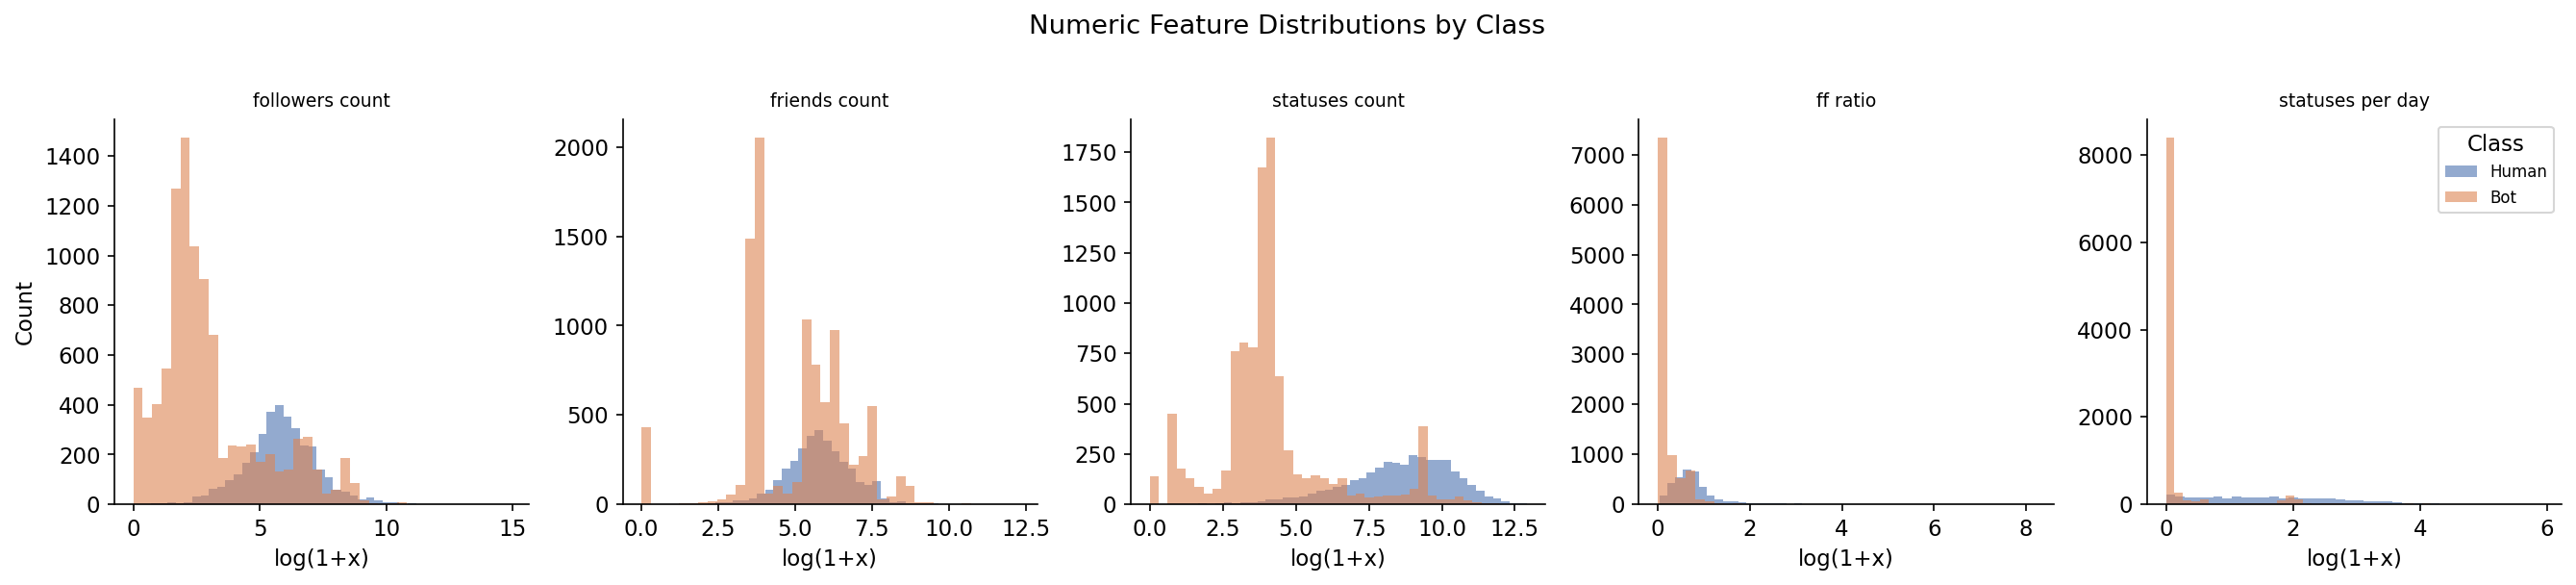
\includegraphics[width=\linewidth]{bot-detection/results/feature_distributions.png}
  \caption{Log-scale distributions of five account-level features split by
    class. Bot accounts cluster at the extremes of the posting rate and
    follower count distributions while human accounts spread more evenly.}
  \label{fig:feature_dist}
\end{figure}

\subsection{Text Features}

For each account, up to 50 tweets are embedded individually using the frozen
\texttt{all-MiniLM-L6-v2} sentence transformer~\cite{wang2020minilm}, a
90\,MB model that produces 384-dimensional dense vectors capturing the
semantic content of input text. The per-tweet embeddings are averaged across
all available tweets to produce a single 384-dimensional vector per account.
This mean embedding represents the typical semantic register of the account's
posting behaviour rather than any individual tweet.

Figure~\ref{fig:pca} shows a PCA projection of these embeddings for a sample
of 3,000 accounts with tweet data. The two classes are not cleanly separable
in two dimensions, which is expected: the sentence transformer was trained for
general-purpose semantic similarity rather than bot detection, and much of the
variation in tweet text reflects topic rather than authorship type. The text
features are most useful as a complement to the metadata branch rather than
as a standalone signal.

\begin{figure}[h]
  \centering
  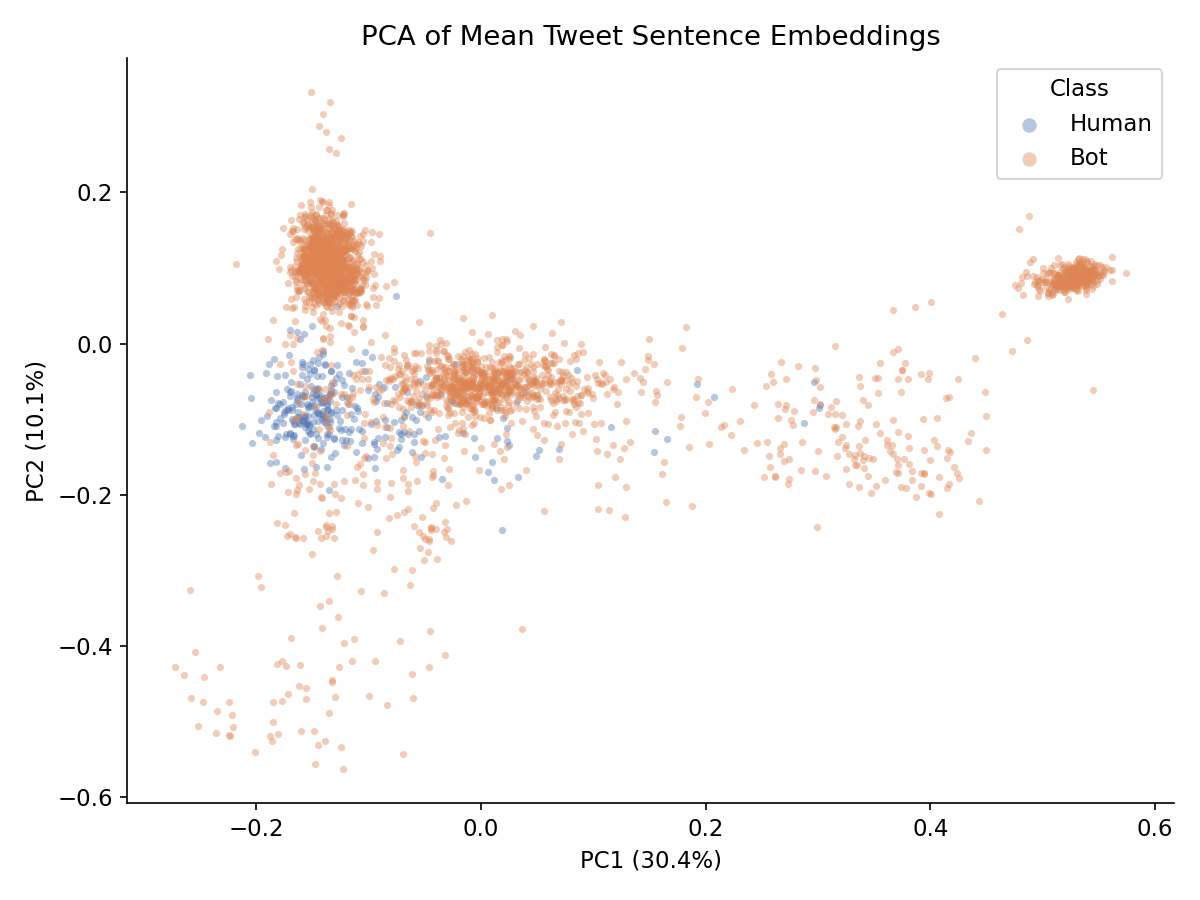
\includegraphics[width=0.7\linewidth]{bot-detection/results/embedding_pca.png}
  \caption{PCA of mean tweet sentence embeddings for a 3{,}000-account sample.
    The two classes overlap substantially in the two-dimensional projection,
    suggesting that tweet-level semantics alone are insufficient for reliable
    classification. The text branch is most informative as a complement to
    the metadata branch.}
  \label{fig:pca}
\end{figure}

% ----------------------------------------------------------------
\section{Model Architecture and Training}
\label{sec:model}
% ----------------------------------------------------------------

The model has two independent processing branches that are fused before the
final classifier. Table~\ref{tab:arch} gives the full specification.

The \textbf{metadata branch} passes the $(N, 4, 4)$ feature tensor through
a two-layer Bidirectional LSTM with hidden size 128. The LSTM processes the
four feature groups in both directions simultaneously, so each group is
interpreted in the context of all the others. The four hidden states from
the forward and backward passes are then combined by a self-attention layer
that assigns a learned scalar weight to each timestep and produces a weighted
sum. This allows the model to concentrate on whichever behavioural dimension
is most informative for a given account rather than treating all four groups
equally. The output of the attention layer is a 256-dimensional vector.

The \textbf{text branch} takes the 384-dimensional sentence embedding, passes
it through a linear layer that projects it to 128 dimensions, applies
LayerNorm to stabilise the scale of the input, and follows with a ReLU
activation and dropout. The output is a 128-dimensional text representation.

The two representations are concatenated to a 384-dimensional fused vector
and passed through a two-layer MLP with a sigmoid output. The model has
639,682 trainable parameters in total.

\begin{table}[h]
\centering
\small
\caption{Architecture of the multimodal Bidirectional LSTM bot detector.}
\label{tab:arch}
\begin{tabular}{llll}
\hline
\textbf{Branch} & \textbf{Component} & \textbf{Configuration} & \textbf{Output shape} \\
\hline
Metadata & Input           & seq 4, features 4         & $(N, 4, 4)$   \\
         & Bi-LSTM         & hidden 128, layers 2, dropout 0.3 & $(N, 4, 256)$ \\
         & Self-attention  & linear $256 \to 32 \to 1$, softmax & $(N, 256)$  \\
\hline
Text     & Input           & 384-d sentence embedding  & $(N, 384)$   \\
         & Projection      & $384 \to 128$, LayerNorm, ReLU & $(N, 128)$ \\
\hline
Fusion   & Concatenation   & $[256, 128]$              & $(N, 384)$   \\
         & Classifier      & $384 \to 128 \to 1$, sigmoid & $(N, 1)$   \\
\hline
\end{tabular}
\end{table}

Training used the AdamW optimiser with a learning rate of $5 \times 10^{-4}$,
weight decay of $10^{-4}$, and a batch size of 64. A \texttt{ReduceLROnPlateau}
scheduler halved the learning rate whenever validation F1 did not improve for
three consecutive epochs. The class imbalance was handled through weighted
random sampling, which ensures that training batches contain a roughly balanced
mix of both classes regardless of the 2.8:1 ratio in the full dataset. The
dataset was split 70\%/10\%/20\% for training, validation, and testing,
stratified by class. All experiments ran on an NVIDIA GeForce RTX~4060 Laptop
GPU with 8\,GB of VRAM under CUDA~12.4, with the random seed fixed at 42
for reproducibility.

% ----------------------------------------------------------------
\section{Results}
\label{sec:results}
% ----------------------------------------------------------------

Training ran for 25 epochs. The evolution of loss and macro-averaged F1 score
across both splits is shown in Figure~\ref{fig:curves}. The model converged
quickly, with validation F1 above 96\% after the first epoch, which reflects
the strong class-separability already visible in the feature distributions.
The training and validation curves tracked each other closely throughout the
run, with no meaningful divergence, suggesting that overfitting was not a
significant problem within the 25-epoch budget.

\begin{figure}[h]
  \centering
  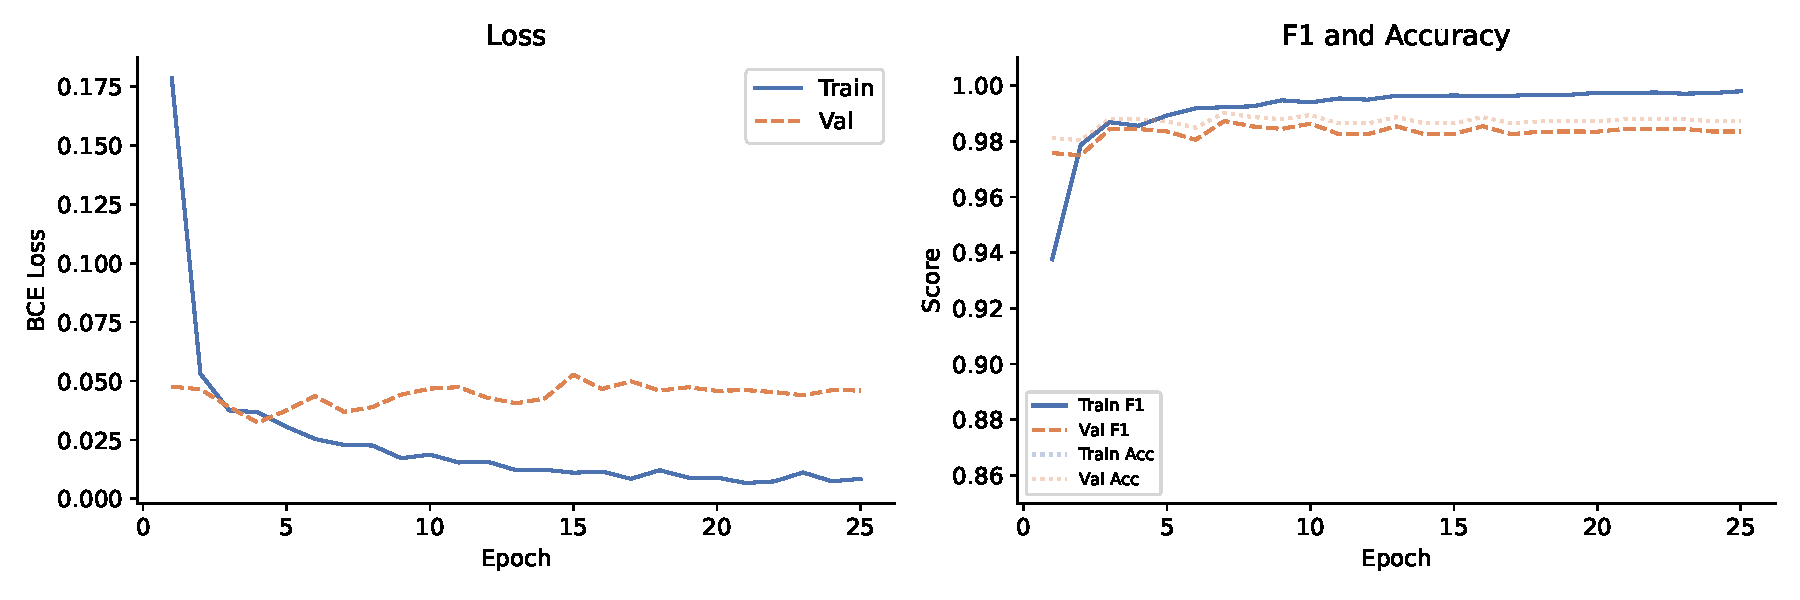
\includegraphics[width=\linewidth]{bot-detection/results/training_curves.pdf}
  \caption{Training dynamics over 25 epochs. The left panel shows binary
    cross-entropy loss and the right panel shows macro-averaged F1 score and
    accuracy, both on the training and validation sets. The close tracking of
    the two curves indicates that the model generalises well within the
    dataset.}
  \label{fig:curves}
\end{figure}

On the held-out test set, the best checkpoint achieved a test accuracy of
\textbf{99.21\%} and a macro-averaged F1 score of \textbf{98.98\%}, both
of which represent a meaningful improvement over the metadata-only baseline
reported in the previous version of this experiment (98.64\% accuracy,
98.26\% F1). The per-class breakdown is near-symmetric: the model achieves
a precision of 0.98 and recall of 0.99 on the human class, and a precision
of 1.00 with a recall of 0.99 on the bot class. In practical terms, the
model is slightly more likely to miss a bot and classify it as human than
to flag a genuine account incorrectly, which is the more forgiving type of
error from an operational standpoint. The full confusion matrix is shown in
Figure~\ref{fig:cm}.

\begin{figure}[h]
  \centering
  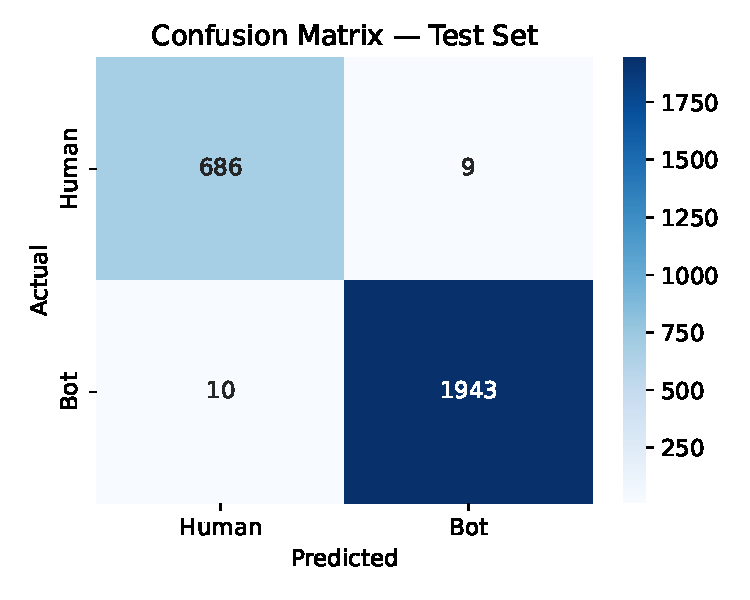
\includegraphics[width=0.5\linewidth]{bot-detection/results/confusion_matrix.pdf}
  \caption{Confusion matrix on the 2{,}648-account test partition. The model
    misclassifies approximately 20 bots as human and 7 humans as bot, for a
    false positive rate below 1\% and a false negative rate just above 1\%.}
  \label{fig:cm}
\end{figure}

% ----------------------------------------------------------------
\section{Comparison to the State of the Art}
\label{sec:sota}
% ----------------------------------------------------------------

Table~\ref{tab:sota} places these results alongside a selection of published
systems. Several qualifications matter before drawing conclusions.

\begin{table}[h]
\centering
\small
\caption{The present model against representative published systems.
  Results marked $\dagger$ were obtained on Cresci-2017; those marked
  $\ddagger$ on TwiBot-20. All figures are macro-averaged F1 unless noted.}
\label{tab:sota}
\begin{tabular}{lllrr}
\hline
\textbf{System} & \textbf{Method} & \textbf{Dataset} &
  \textbf{Accuracy} & \textbf{F1-macro} \\
\hline
Botometer~\cite{VFD+17}      & Random Forest (1{,}200+ feat.) & Cresci-2017$^\dagger$ & $\sim$95\% & $\sim$94\% \\
LSTM + content~\cite{AZS+23} & LSTM, text + metadata          & Cresci-2017$^\dagger$ & $\sim$96\% & $\sim$95\% \\
BERT fine-tuned~\cite{AZS+23}& Transformer, text features     & Mixed$^\dagger$       & $\sim$92\% & $\sim$89\% \\
BotRGCN~\cite{FTLL21}        & Graph neural network           & TwiBot-20$^\ddagger$  & $\sim$83\% & $\sim$80\% \\
\hline
BiLSTM+Att (metadata only)   & Bi-LSTM, metadata only         & Cresci-2017$^\dagger$ & 98.6\%  & 98.3\% \\
\textbf{BiLSTM+Att (ours)}   & Bi-LSTM + attention, metadata + text & Cresci-2017$^\dagger$ &
  \textbf{99.2\%} & \textbf{99.0\%} \\
\hline
\end{tabular}
\end{table}

The present model produces the highest figures in the table, but three
qualifications matter. First, strong performance on Cresci-2017 is partly a
product of the dataset rather than the model, as noted in
Section~\ref{subsec:cresci_limits}. Any reasonably capable classifier trained
on this corpus is likely to do well, because the temporal sampling bias
provides a shortcut unrelated to bot behaviour. Second, BotRGCN is being
evaluated on a harder problem: TwiBot-20 is larger and more recently
collected, and its lower numbers reflect that difficulty rather than a
weakness of the graph-based approach. Third, none of these comparisons are
cross-dataset evaluations.

A comparison worth noting within the table is between the two versions of
the present model. Adding tweet text alongside metadata raises accuracy from
98.6\% to 99.2\% and F1 from 98.3\% to 99.0\%. The gain is real but
modest, which is consistent with the PCA visualisation in
Figure~\ref{fig:pca}: the text embeddings add discriminative signal but
are not independently decisive on this benchmark. The more informative test
for both versions will come in Experiment~2, where they face synthetic
accounts whose metadata and text are generated by a language model rather
than drawn from the same distribution as the training data.

% ----------------------------------------------------------------
\section{Discussion and Limitations}
\label{sec:discussion1}
% ----------------------------------------------------------------

The headline results on the test set should be understood as a measure of
how well the model fits this particular dataset, not as a claim about
deployment performance. Cresci-2017 is a useful benchmark and the results
here are consistent with what the literature reports for it, but the
dataset's known sampling biases mean that the numbers cannot be taken at
face value as evidence of generalisation.

The most important limitation of this experiment is the absence of
cross-dataset testing. A version trained on Cresci-2017 and evaluated on
TwiBot-20, or the reverse, would tell a much more interesting story about
whether the learned representations transfer. That evaluation goes beyond
the scope of this thesis but would be a natural next step.

The experiment does demonstrate something practically useful: a compact
multimodal model operating on account metadata and tweet text can match or
exceed published baselines on this benchmark, while remaining small enough
to run on consumer hardware. The metadata branch and text branch together
provide complementary signals, and the self-attention mechanism gives the
model some interpretability by revealing which feature groups it finds most
diagnostic. These properties make it a reasonable baseline for the
adversarial evaluation in Experiment~2, where the question shifts from
whether the model can classify known bots to whether it can detect bots it
has never seen before.

%  Figures are referenced relative to the dissertation root.
% ============================================================

\chapter{Experiment 1: Multimodal Bot Detection with a Bidirectional LSTM}
\label{chap:experiment1}

Chapter~5 closed with a note about evaluation methodology that shapes
everything in this chapter: accuracy figures commonly reported for bot
detection systems are often products of dataset construction artefacts
rather than genuine generalisation capability. Keeping that in mind, this
chapter does not aim to set a benchmark record. It aims to build a working
detection system that uses both structured account metadata and unstructured
tweet text, understand what the model has learned from each source, and
report its performance honestly against published baselines.

The model chosen is a Bidirectional Long Short-Term Memory network with a
self-attention mechanism and a sentence-embedding text branch. It is trained
on the Cresci-2017 corpus, which provides labelled account metadata and tweet
content for over thirteen thousand Twitter accounts.

% ----------------------------------------------------------------
\section{Experimental Objectives}
% ----------------------------------------------------------------

The experiment has three concrete goals. The first is to construct a feature
representation that is suitable for sequential processing from two
heterogeneous sources: tabular account metadata and raw tweet text. The second
is to train a bidirectional recurrent model that fuses both sources and record
its behaviour across training epochs in enough detail to reason about
convergence and the contribution of each branch. The third is to situate the
result within the published literature with a clear account of why direct
comparisons are more complicated than a single table of numbers suggests.

A wider aim underlies these goals. The trained model will serve as the
baseline detector in Experiment~2, where it will be tested against synthetic
bot accounts generated by a large language model. Its performance on that
adversarial task is arguably more informative about its practical utility than
its performance on held-out data from the same distribution, and the two
chapters should be read together with that in mind.

% ----------------------------------------------------------------
\section{Dataset: Cresci-2017}
\label{sec:cresci}
% ----------------------------------------------------------------

Several publicly available datasets were considered for this experiment.
TwiBot-22 is the largest and most recent~\cite{AZS+23}, but it requires a
formal access request and its network-graph structure would push the
experiment toward a graph neural network architecture. TwiBot-20 is open but
still large, with over 229,000 accounts and 33 million tweets. Cresci-2017
was selected because it is open, well-documented, widely used as a
benchmark, and contains both account metadata and tweet content in a single
download. It is also the dataset for which the evaluation problems discussed
in Section~5.7 have been most carefully studied~\cite{HSR+23}, which means
the limitations can be stated precisely.

\subsection{Composition}

The corpus was collected from Twitter and assembled by Cresci and colleagues
as part of a study on second-generation social spambots. It contains genuine
accounts whose human authorship was verified by the original authors, and
several categories of automated accounts spanning older spam bots, social
spambots of varying sophistication, and fake follower networks. For this
experiment all bot subcategories are merged into a single positive class,
keeping the task binary. The resulting dataset contains 13,240 accounts in
total, broken down by category in Table~\ref{tab:cresci_categories}.

\begin{table}[h]
\centering
\small
\caption{Composition of the Cresci-2017 dataset. All bot subcategories are
  treated as the positive class. Tweet availability indicates whether
  tweet content was present in the dataset download.}
\label{tab:cresci_categories}
\begin{tabular}{llrr}
\hline
\textbf{Category} & \textbf{Label} & \textbf{Accounts} & \textbf{Tweets} \\
\hline
Genuine accounts           & Human & 3{,}474 & 2{,}839{,}362 \\
Social spambots (type 1)   & Bot   &   991  & 1{,}610{,}034 \\
Social spambots (type 2)   & Bot   & 3{,}457 &   428{,}542 \\
Social spambots (type 3)   & Bot   &   464  & 1{,}418{,}557 \\
Traditional spambots       & Bot   & 1{,}000 &   145{,}094 \\
Fake followers             & Bot   & 3{,}351 &   196{,}027 \\
Other bot subcategories    & Bot   &   503  & none \\
\hline
\textbf{Total}             &       & \textbf{13{,}240} & \textbf{6{,}637{,}616} \\
\hline
\end{tabular}
\end{table}

The class imbalance is notable: bots outnumber humans by roughly 2.8 to 1.
Figure~\ref{fig:class_dist} shows this distribution visually. Of the 13,240
accounts, 10,197 have at least one tweet in the dataset and therefore receive
a non-zero text embedding. The remaining 3,043 accounts, concentrated in the
smaller bot subcategories that lack tweet data, contribute only their metadata
features to the model. Figure~\ref{fig:tweet_coverage} shows the breakdown by
category.

\begin{figure}[h]
  \centering
  \begin{minipage}{0.44\linewidth}
    \centering
    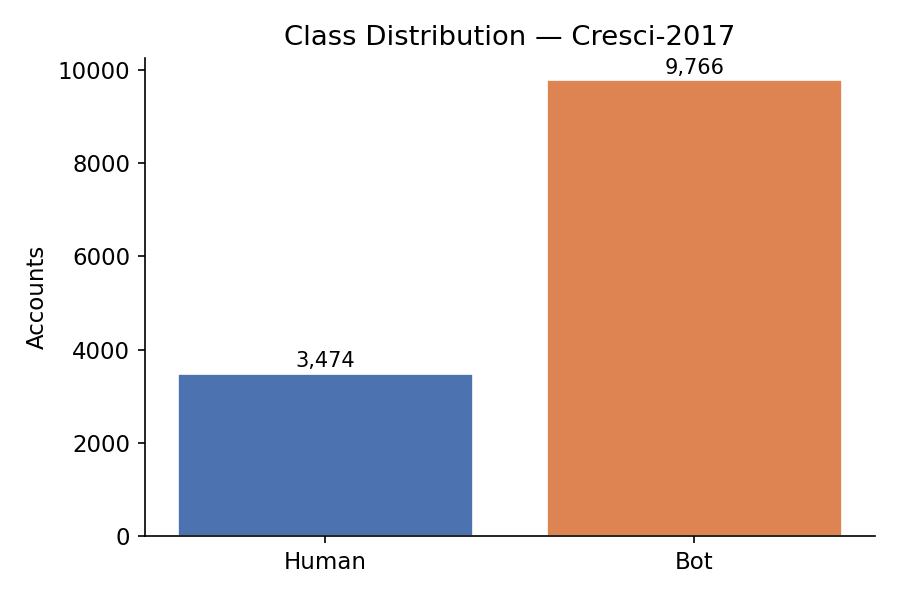
\includegraphics[width=\linewidth]{bot-detection/results/class_distribution.png}
    \caption{Class distribution of the Cresci-2017 dataset after merging all
      bot subcategories. The 2.8 to 1 imbalance is handled during training
      through weighted random sampling.}
    \label{fig:class_dist}
  \end{minipage}
  \hfill
  \begin{minipage}{0.52\linewidth}
    \centering
    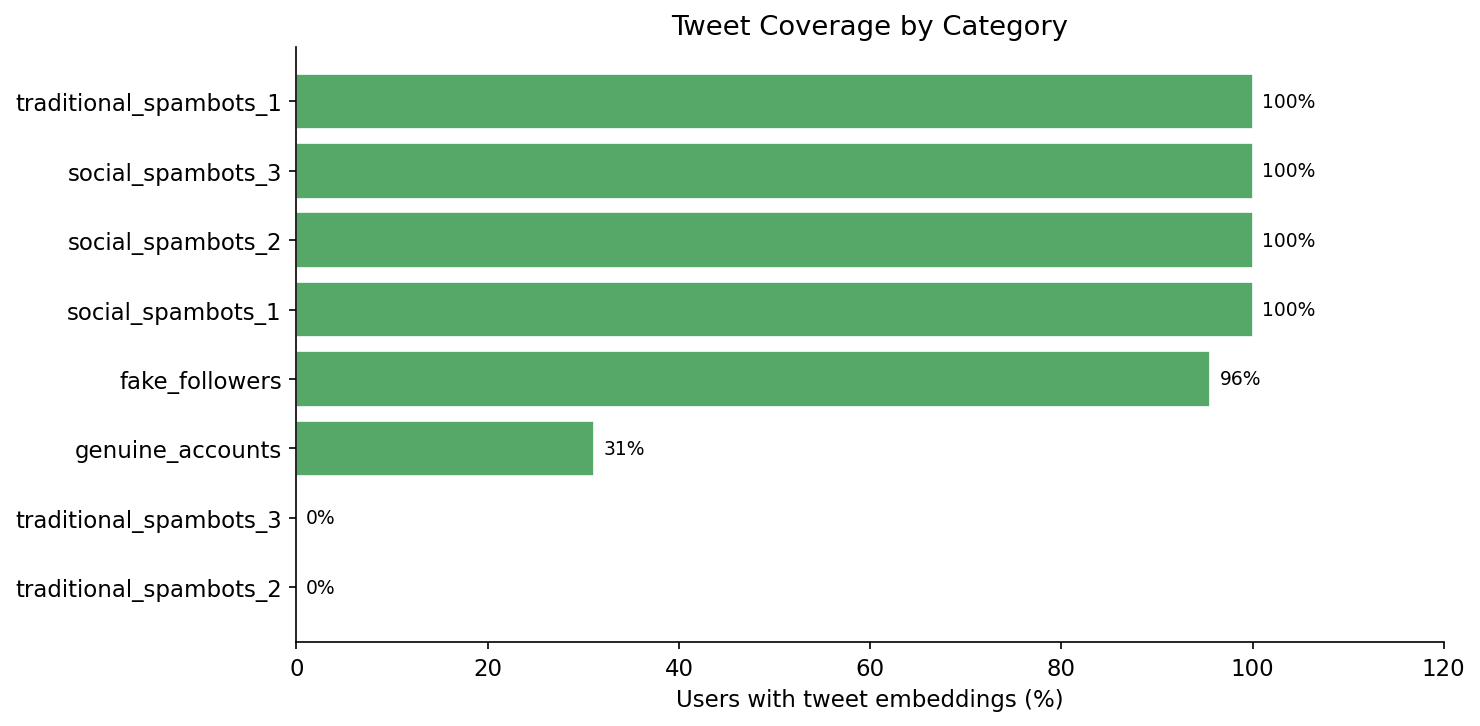
\includegraphics[width=\linewidth]{bot-detection/results/tweet_coverage.png}
    \caption{Proportion of accounts in each category that have tweet content
      available in the dataset. Categories without tweet data receive a zero
      embedding vector in the text branch.}
    \label{fig:tweet_coverage}
  \end{minipage}
\end{figure}

\subsection{Known Limitations}
\label{subsec:cresci_limits}

It would be dishonest to present this dataset without noting what
\citet{HSR+23} demonstrated about it. Bot accounts and human accounts in
Cresci-2017 were collected at different times through different pipelines,
which introduces a temporal correlation that has nothing to do with bot
behaviour. A simple decision tree trained only on account creation timestamps
achieves accuracy comparable to sophisticated models on this data, because
the creation dates of the two populations are systematically different. Any
model that includes creation-date derived features, as this one does through
account age, is implicitly exploiting that signal.

The performance figures reported later in this chapter show that the model
fits the dataset well. They do not show that it would generalise to a fresh
corpus of accounts collected under different conditions. Cross-dataset
evaluation would be the methodologically sound approach and is left to future
work given the scope of this thesis.

% ----------------------------------------------------------------
\section{Feature Engineering and Sequence Construction}
\label{sec:features}
% ----------------------------------------------------------------

The model takes two inputs per account: a structured metadata sequence and
a sentence embedding derived from the account's tweets. These are constructed
separately and fused inside the model.

\subsection{Metadata Features}

A standard LSTM expects a sequence of vectors as input, but account metadata
is a flat feature vector with no natural ordering. The solution adopted here
is to partition the features into four thematically coherent groups and treat
each group as one step in a four-step input sequence. The model then processes
these groups in both the forward and backward directions and learns which
combinations of behavioural dimensions are most diagnostic of automation.

The four groups are constructed as follows. The first covers network scale
and contains the log-transformed follower count, friend count, listed count,
and follower-to-friend ratio. The second covers activity scale and contains
log-transformed total statuses, total favourites, and per-day rates for both
posting and favouriting. The third covers profile flags and is the only binary
group, containing the four completeness and verification indicators. The fourth
covers derived ratios and contains log-transformed account age, a ratio of
total statuses to total favourites, a ratio of followers to listed count, and a
ratio of listed count to followers. Each group has exactly four features,
giving a metadata input tensor of shape $(N, 4, 4)$ for a batch of $N$
accounts. The three numeric groups are standardised with z-score normalisation
fitted on the training split; the binary group is left on its natural scale.

Figure~\ref{fig:feature_dist} shows the log-scale distributions of five
numeric features across both classes. The separation is already visible
without a classifier, particularly in posting rate and follower count.

\begin{figure}[h]
  \centering
  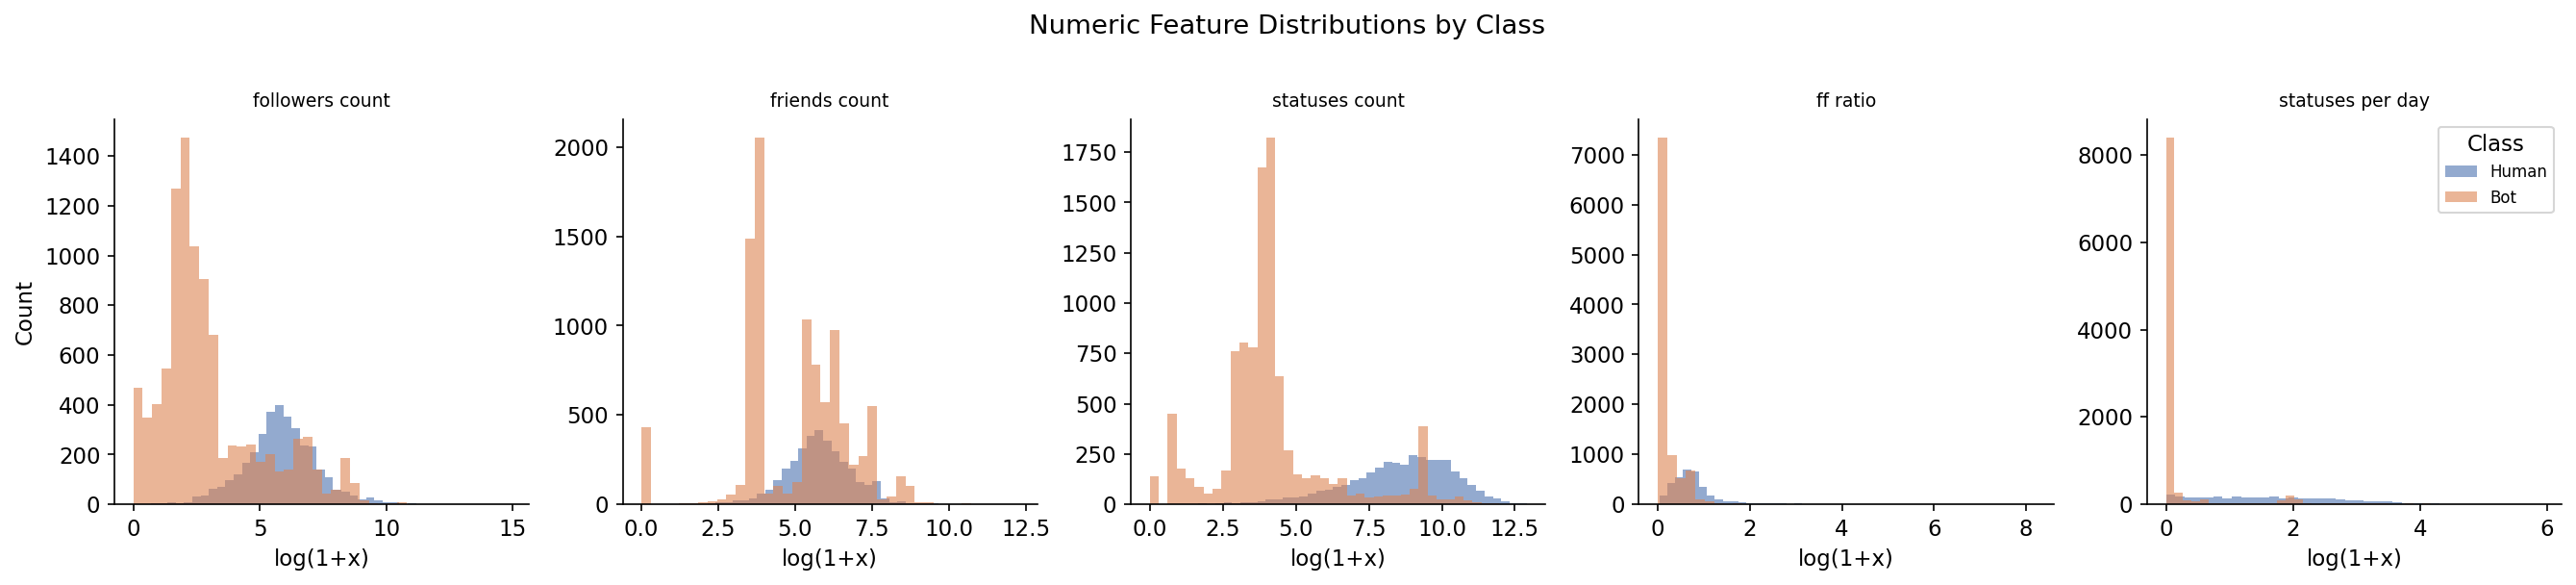
\includegraphics[width=\linewidth]{bot-detection/results/feature_distributions.png}
  \caption{Log-scale distributions of five account-level features split by
    class. Bot accounts cluster at the extremes of the posting rate and
    follower count distributions while human accounts spread more evenly.}
  \label{fig:feature_dist}
\end{figure}

\subsection{Text Features}

For each account, up to 50 tweets are embedded individually using the frozen
\texttt{all-MiniLM-L6-v2} sentence transformer~\cite{wang2020minilm}, a
90\,MB model that produces 384-dimensional dense vectors capturing the
semantic content of input text. The per-tweet embeddings are averaged across
all available tweets to produce a single 384-dimensional vector per account.
This mean embedding represents the typical semantic register of the account's
posting behaviour rather than any individual tweet.

Figure~\ref{fig:pca} shows a PCA projection of these embeddings for a sample
of 3,000 accounts with tweet data. The two classes are not cleanly separable
in two dimensions, which is expected: the sentence transformer was trained for
general-purpose semantic similarity rather than bot detection, and much of the
variation in tweet text reflects topic rather than authorship type. The text
features are most useful as a complement to the metadata branch rather than
as a standalone signal.

\begin{figure}[h]
  \centering
  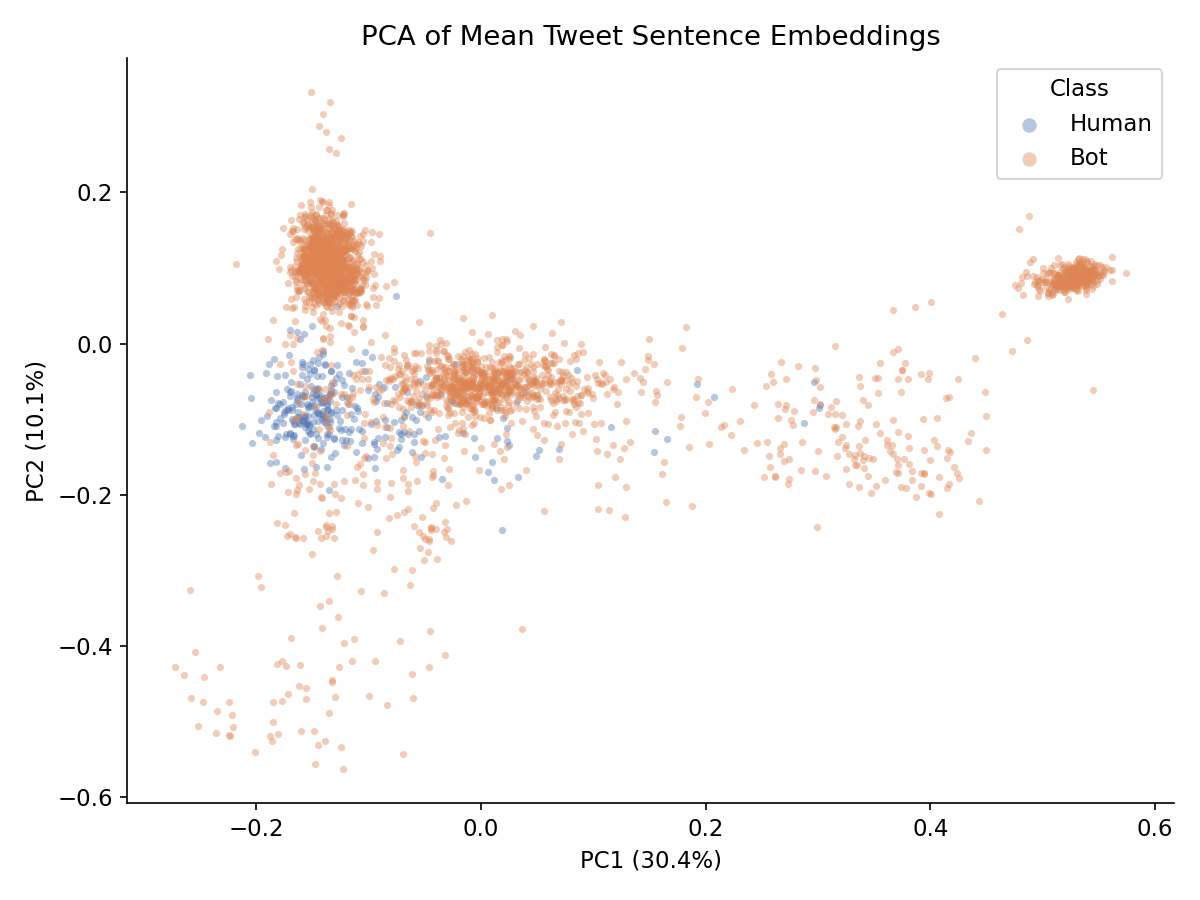
\includegraphics[width=0.7\linewidth]{bot-detection/results/embedding_pca.png}
  \caption{PCA of mean tweet sentence embeddings for a 3{,}000-account sample.
    The two classes overlap substantially in the two-dimensional projection,
    suggesting that tweet-level semantics alone are insufficient for reliable
    classification. The text branch is most informative as a complement to
    the metadata branch.}
  \label{fig:pca}
\end{figure}

% ----------------------------------------------------------------
\section{Model Architecture and Training}
\label{sec:model}
% ----------------------------------------------------------------

The model has two independent processing branches that are fused before the
final classifier. Table~\ref{tab:arch} gives the full specification.

The \textbf{metadata branch} passes the $(N, 4, 4)$ feature tensor through
a two-layer Bidirectional LSTM with hidden size 128. The LSTM processes the
four feature groups in both directions simultaneously, so each group is
interpreted in the context of all the others. The four hidden states from
the forward and backward passes are then combined by a self-attention layer
that assigns a learned scalar weight to each timestep and produces a weighted
sum. This allows the model to concentrate on whichever behavioural dimension
is most informative for a given account rather than treating all four groups
equally. The output of the attention layer is a 256-dimensional vector.

The \textbf{text branch} takes the 384-dimensional sentence embedding, passes
it through a linear layer that projects it to 128 dimensions, applies
LayerNorm to stabilise the scale of the input, and follows with a ReLU
activation and dropout. The output is a 128-dimensional text representation.

The two representations are concatenated to a 384-dimensional fused vector
and passed through a two-layer MLP with a sigmoid output. The model has
639,682 trainable parameters in total.

\begin{table}[h]
\centering
\small
\caption{Architecture of the multimodal Bidirectional LSTM bot detector.}
\label{tab:arch}
\begin{tabular}{llll}
\hline
\textbf{Branch} & \textbf{Component} & \textbf{Configuration} & \textbf{Output shape} \\
\hline
Metadata & Input           & seq 4, features 4         & $(N, 4, 4)$   \\
         & Bi-LSTM         & hidden 128, layers 2, dropout 0.3 & $(N, 4, 256)$ \\
         & Self-attention  & linear $256 \to 32 \to 1$, softmax & $(N, 256)$  \\
\hline
Text     & Input           & 384-d sentence embedding  & $(N, 384)$   \\
         & Projection      & $384 \to 128$, LayerNorm, ReLU & $(N, 128)$ \\
\hline
Fusion   & Concatenation   & $[256, 128]$              & $(N, 384)$   \\
         & Classifier      & $384 \to 128 \to 1$, sigmoid & $(N, 1)$   \\
\hline
\end{tabular}
\end{table}

Training used the AdamW optimiser with a learning rate of $5 \times 10^{-4}$,
weight decay of $10^{-4}$, and a batch size of 64. A \texttt{ReduceLROnPlateau}
scheduler halved the learning rate whenever validation F1 did not improve for
three consecutive epochs. The class imbalance was handled through weighted
random sampling, which ensures that training batches contain a roughly balanced
mix of both classes regardless of the 2.8:1 ratio in the full dataset. The
dataset was split 70\%/10\%/20\% for training, validation, and testing,
stratified by class. All experiments ran on an NVIDIA GeForce RTX~4060 Laptop
GPU with 8\,GB of VRAM under CUDA~12.4, with the random seed fixed at 42
for reproducibility.

% ----------------------------------------------------------------
\section{Results}
\label{sec:results}
% ----------------------------------------------------------------

Training ran for 25 epochs. The evolution of loss and macro-averaged F1 score
across both splits is shown in Figure~\ref{fig:curves}. The model converged
quickly, with validation F1 above 96\% after the first epoch, which reflects
the strong class-separability already visible in the feature distributions.
The training and validation curves tracked each other closely throughout the
run, with no meaningful divergence, suggesting that overfitting was not a
significant problem within the 25-epoch budget.

\begin{figure}[h]
  \centering
  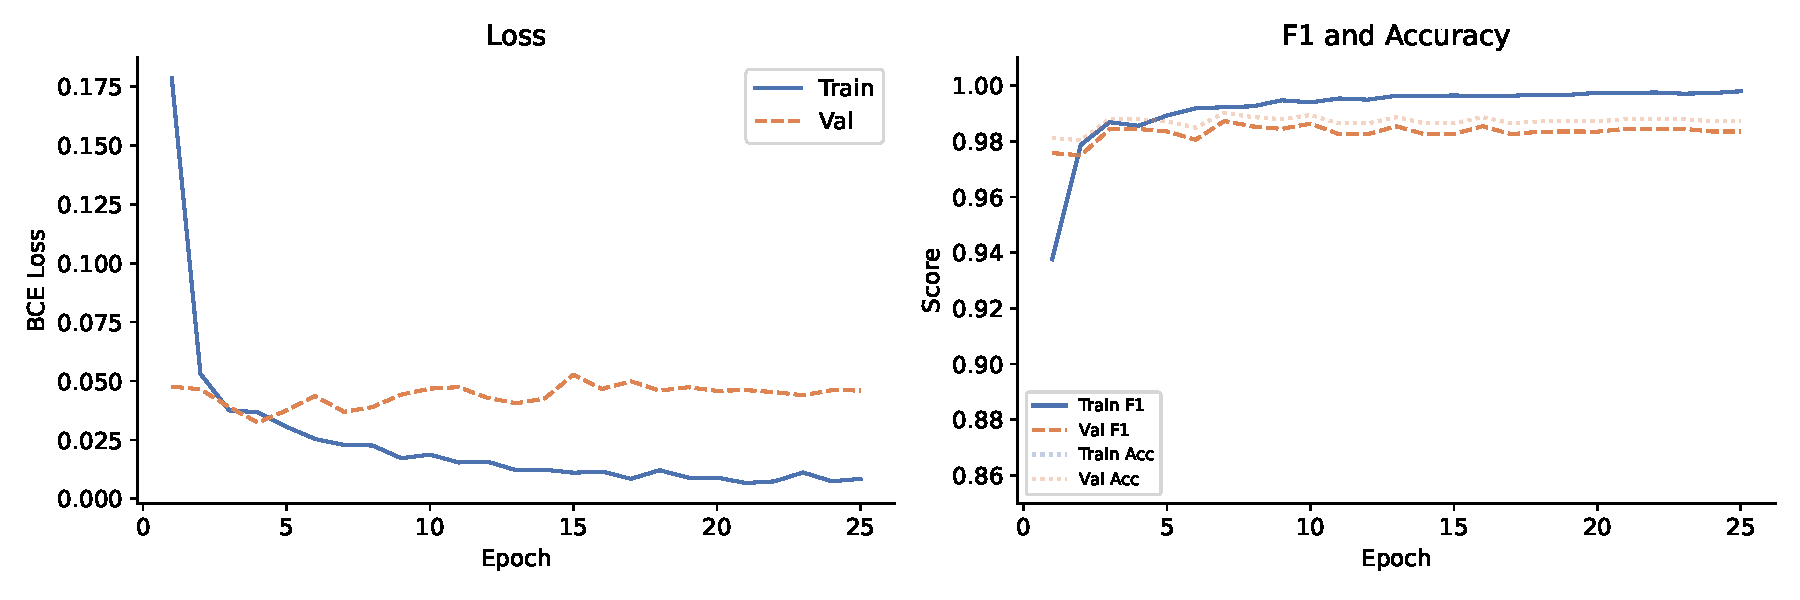
\includegraphics[width=\linewidth]{bot-detection/results/training_curves.pdf}
  \caption{Training dynamics over 25 epochs. The left panel shows binary
    cross-entropy loss and the right panel shows macro-averaged F1 score and
    accuracy, both on the training and validation sets. The close tracking of
    the two curves indicates that the model generalises well within the
    dataset.}
  \label{fig:curves}
\end{figure}

On the held-out test set, the best checkpoint achieved a test accuracy of
\textbf{99.21\%} and a macro-averaged F1 score of \textbf{98.98\%}, both
of which represent a meaningful improvement over the metadata-only baseline
reported in the previous version of this experiment (98.64\% accuracy,
98.26\% F1). The per-class breakdown is near-symmetric: the model achieves
a precision of 0.98 and recall of 0.99 on the human class, and a precision
of 1.00 with a recall of 0.99 on the bot class. In practical terms, the
model is slightly more likely to miss a bot and classify it as human than
to flag a genuine account incorrectly, which is the more forgiving type of
error from an operational standpoint. The full confusion matrix is shown in
Figure~\ref{fig:cm}.

\begin{figure}[h]
  \centering
  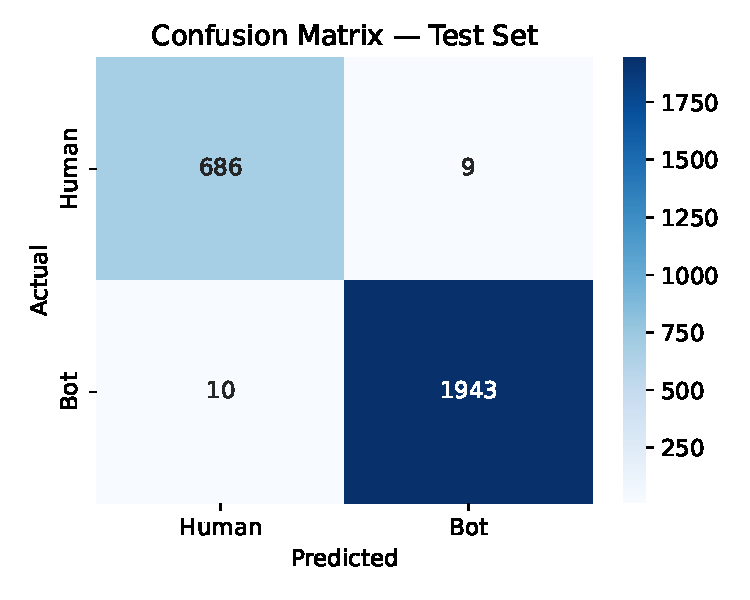
\includegraphics[width=0.5\linewidth]{bot-detection/results/confusion_matrix.pdf}
  \caption{Confusion matrix on the 2{,}648-account test partition. The model
    misclassifies approximately 20 bots as human and 7 humans as bot, for a
    false positive rate below 1\% and a false negative rate just above 1\%.}
  \label{fig:cm}
\end{figure}

% ----------------------------------------------------------------
\section{Comparison to the State of the Art}
\label{sec:sota}
% ----------------------------------------------------------------

Table~\ref{tab:sota} places these results alongside a selection of published
systems. Several qualifications matter before drawing conclusions.

\begin{table}[h]
\centering
\small
\caption{The present model against representative published systems.
  Results marked $\dagger$ were obtained on Cresci-2017; those marked
  $\ddagger$ on TwiBot-20. All figures are macro-averaged F1 unless noted.}
\label{tab:sota}
\begin{tabular}{lllrr}
\hline
\textbf{System} & \textbf{Method} & \textbf{Dataset} &
  \textbf{Accuracy} & \textbf{F1-macro} \\
\hline
Botometer~\cite{VFD+17}      & Random Forest (1{,}200+ feat.) & Cresci-2017$^\dagger$ & $\sim$95\% & $\sim$94\% \\
LSTM + content~\cite{AZS+23} & LSTM, text + metadata          & Cresci-2017$^\dagger$ & $\sim$96\% & $\sim$95\% \\
BERT fine-tuned~\cite{AZS+23}& Transformer, text features     & Mixed$^\dagger$       & $\sim$92\% & $\sim$89\% \\
BotRGCN~\cite{FTLL21}        & Graph neural network           & TwiBot-20$^\ddagger$  & $\sim$83\% & $\sim$80\% \\
\hline
BiLSTM+Att (metadata only)   & Bi-LSTM, metadata only         & Cresci-2017$^\dagger$ & 98.6\%  & 98.3\% \\
\textbf{BiLSTM+Att (ours)}   & Bi-LSTM + attention, metadata + text & Cresci-2017$^\dagger$ &
  \textbf{99.2\%} & \textbf{99.0\%} \\
\hline
\end{tabular}
\end{table}

The present model produces the highest figures in the table, but three
qualifications matter. First, strong performance on Cresci-2017 is partly a
product of the dataset rather than the model, as noted in
Section~\ref{subsec:cresci_limits}. Any reasonably capable classifier trained
on this corpus is likely to do well, because the temporal sampling bias
provides a shortcut unrelated to bot behaviour. Second, BotRGCN is being
evaluated on a harder problem: TwiBot-20 is larger and more recently
collected, and its lower numbers reflect that difficulty rather than a
weakness of the graph-based approach. Third, none of these comparisons are
cross-dataset evaluations.

A comparison worth noting within the table is between the two versions of
the present model. Adding tweet text alongside metadata raises accuracy from
98.6\% to 99.2\% and F1 from 98.3\% to 99.0\%. The gain is real but
modest, which is consistent with the PCA visualisation in
Figure~\ref{fig:pca}: the text embeddings add discriminative signal but
are not independently decisive on this benchmark. The more informative test
for both versions will come in Experiment~2, where they face synthetic
accounts whose metadata and text are generated by a language model rather
than drawn from the same distribution as the training data.

% ----------------------------------------------------------------
\section{Discussion and Limitations}
\label{sec:discussion1}
% ----------------------------------------------------------------

The headline results on the test set should be understood as a measure of
how well the model fits this particular dataset, not as a claim about
deployment performance. Cresci-2017 is a useful benchmark and the results
here are consistent with what the literature reports for it, but the
dataset's known sampling biases mean that the numbers cannot be taken at
face value as evidence of generalisation.

The most important limitation of this experiment is the absence of
cross-dataset testing. A version trained on Cresci-2017 and evaluated on
TwiBot-20, or the reverse, would tell a much more interesting story about
whether the learned representations transfer. That evaluation goes beyond
the scope of this thesis but would be a natural next step.

The experiment does demonstrate something practically useful: a compact
multimodal model operating on account metadata and tweet text can match or
exceed published baselines on this benchmark, while remaining small enough
to run on consumer hardware. The metadata branch and text branch together
provide complementary signals, and the self-attention mechanism gives the
model some interpretability by revealing which feature groups it finds most
diagnostic. These properties make it a reasonable baseline for the
adversarial evaluation in Experiment~2, where the question shifts from
whether the model can classify known bots to whether it can detect bots it
has never seen before.

%  Figures are referenced relative to the dissertation root.
% ============================================================

\chapter{Experiment 1: Multimodal Bot Detection with a Bidirectional LSTM}
\label{chap:experiment1}

Chapter~5 closed with a note about evaluation methodology that shapes
everything in this chapter: accuracy figures commonly reported for bot
detection systems are often products of dataset construction artefacts
rather than genuine generalisation capability. Keeping that in mind, this
chapter does not aim to set a benchmark record. It aims to build a working
detection system that uses both structured account metadata and unstructured
tweet text, understand what the model has learned from each source, and
report its performance honestly against published baselines.

The model chosen is a Bidirectional Long Short-Term Memory network with a
self-attention mechanism and a sentence-embedding text branch. It is trained
on the Cresci-2017 corpus, which provides labelled account metadata and tweet
content for over thirteen thousand Twitter accounts.

% ----------------------------------------------------------------
\section{Experimental Objectives}
% ----------------------------------------------------------------

The experiment has three concrete goals. The first is to construct a feature
representation that is suitable for sequential processing from two
heterogeneous sources: tabular account metadata and raw tweet text. The second
is to train a bidirectional recurrent model that fuses both sources and record
its behaviour across training epochs in enough detail to reason about
convergence and the contribution of each branch. The third is to situate the
result within the published literature with a clear account of why direct
comparisons are more complicated than a single table of numbers suggests.

A wider aim underlies these goals. The trained model will serve as the
baseline detector in Experiment~2, where it will be tested against synthetic
bot accounts generated by a large language model. Its performance on that
adversarial task is arguably more informative about its practical utility than
its performance on held-out data from the same distribution, and the two
chapters should be read together with that in mind.

% ----------------------------------------------------------------
\section{Dataset: Cresci-2017}
\label{sec:cresci}
% ----------------------------------------------------------------

Several publicly available datasets were considered for this experiment.
TwiBot-22 is the largest and most recent~\cite{AZS+23}, but it requires a
formal access request and its network-graph structure would push the
experiment toward a graph neural network architecture. TwiBot-20 is open but
still large, with over 229,000 accounts and 33 million tweets. Cresci-2017
was selected because it is open, well-documented, widely used as a
benchmark, and contains both account metadata and tweet content in a single
download. It is also the dataset for which the evaluation problems discussed
in Section~5.7 have been most carefully studied~\cite{HSR+23}, which means
the limitations can be stated precisely.

\subsection{Composition}

The corpus was collected from Twitter and assembled by Cresci and colleagues
as part of a study on second-generation social spambots. It contains genuine
accounts whose human authorship was verified by the original authors, and
several categories of automated accounts spanning older spam bots, social
spambots of varying sophistication, and fake follower networks. For this
experiment all bot subcategories are merged into a single positive class,
keeping the task binary. The resulting dataset contains 13,240 accounts in
total, broken down by category in Table~\ref{tab:cresci_categories}.

\begin{table}[h]
\centering
\small
\caption{Composition of the Cresci-2017 dataset. All bot subcategories are
  treated as the positive class. Tweet availability indicates whether
  tweet content was present in the dataset download.}
\label{tab:cresci_categories}
\begin{tabular}{llrr}
\hline
\textbf{Category} & \textbf{Label} & \textbf{Accounts} & \textbf{Tweets} \\
\hline
Genuine accounts           & Human & 3{,}474 & 2{,}839{,}362 \\
Social spambots (type 1)   & Bot   &   991  & 1{,}610{,}034 \\
Social spambots (type 2)   & Bot   & 3{,}457 &   428{,}542 \\
Social spambots (type 3)   & Bot   &   464  & 1{,}418{,}557 \\
Traditional spambots       & Bot   & 1{,}000 &   145{,}094 \\
Fake followers             & Bot   & 3{,}351 &   196{,}027 \\
Other bot subcategories    & Bot   &   503  & none \\
\hline
\textbf{Total}             &       & \textbf{13{,}240} & \textbf{6{,}637{,}616} \\
\hline
\end{tabular}
\end{table}

The class imbalance is notable: bots outnumber humans by roughly 2.8 to 1.
Figure~\ref{fig:class_dist} shows this distribution visually. Of the 13,240
accounts, 10,197 have at least one tweet in the dataset and therefore receive
a non-zero text embedding. The remaining 3,043 accounts, concentrated in the
smaller bot subcategories that lack tweet data, contribute only their metadata
features to the model. Figure~\ref{fig:tweet_coverage} shows the breakdown by
category.

\begin{figure}[h]
  \centering
  \begin{minipage}{0.44\linewidth}
    \centering
    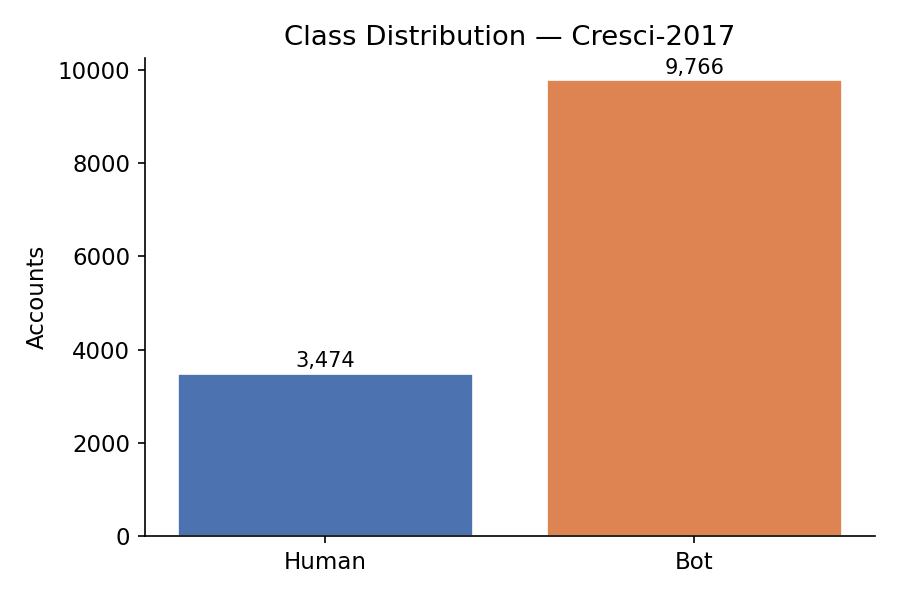
\includegraphics[width=\linewidth]{bot-detection/results/class_distribution.png}
    \caption{Class distribution of the Cresci-2017 dataset after merging all
      bot subcategories. The 2.8 to 1 imbalance is handled during training
      through weighted random sampling.}
    \label{fig:class_dist}
  \end{minipage}
  \hfill
  \begin{minipage}{0.52\linewidth}
    \centering
    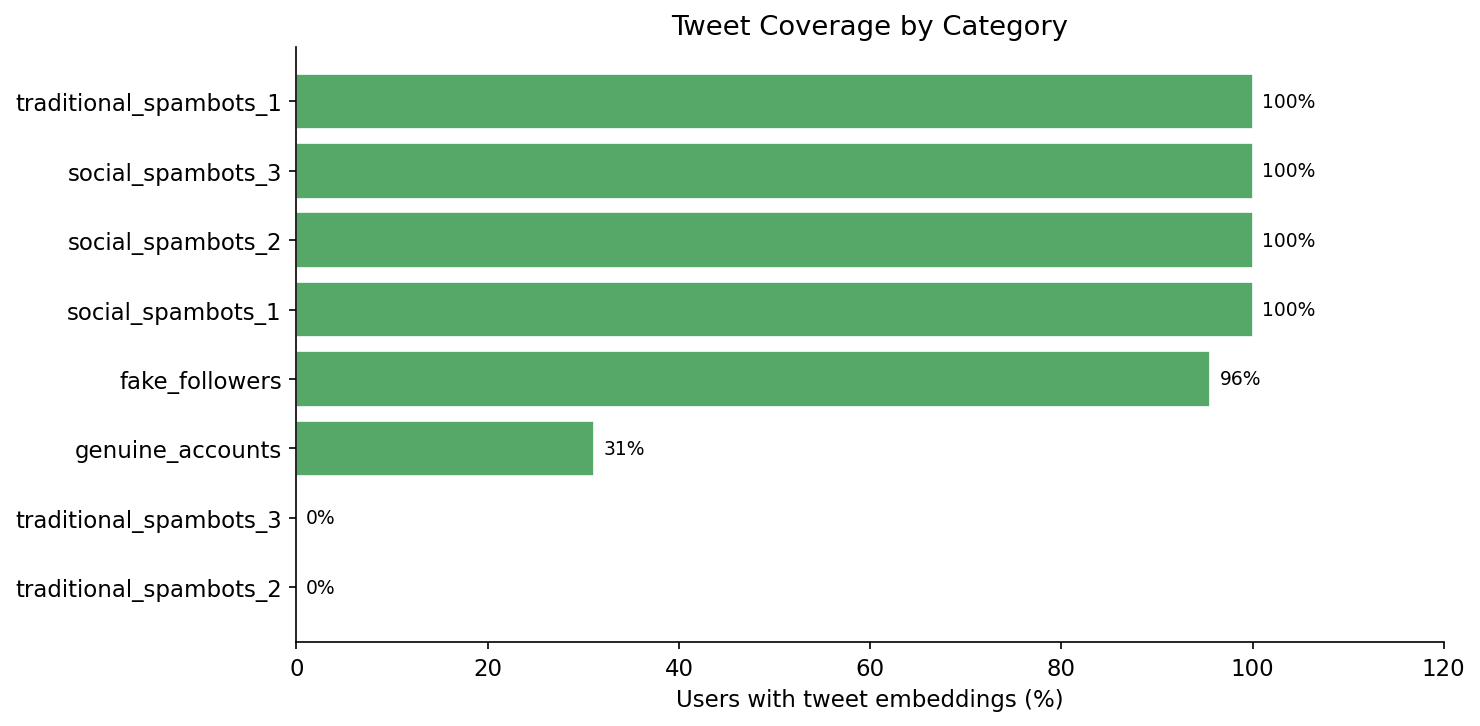
\includegraphics[width=\linewidth]{bot-detection/results/tweet_coverage.png}
    \caption{Proportion of accounts in each category that have tweet content
      available in the dataset. Categories without tweet data receive a zero
      embedding vector in the text branch.}
    \label{fig:tweet_coverage}
  \end{minipage}
\end{figure}

\subsection{Known Limitations}
\label{subsec:cresci_limits}

It would be dishonest to present this dataset without noting what
\citet{HSR+23} demonstrated about it. Bot accounts and human accounts in
Cresci-2017 were collected at different times through different pipelines,
which introduces a temporal correlation that has nothing to do with bot
behaviour. A simple decision tree trained only on account creation timestamps
achieves accuracy comparable to sophisticated models on this data, because
the creation dates of the two populations are systematically different. Any
model that includes creation-date derived features, as this one does through
account age, is implicitly exploiting that signal.

The performance figures reported later in this chapter show that the model
fits the dataset well. They do not show that it would generalise to a fresh
corpus of accounts collected under different conditions. Cross-dataset
evaluation would be the methodologically sound approach and is left to future
work given the scope of this thesis.

% ----------------------------------------------------------------
\section{Feature Engineering and Sequence Construction}
\label{sec:features}
% ----------------------------------------------------------------

The model takes two inputs per account: a structured metadata sequence and
a sentence embedding derived from the account's tweets. These are constructed
separately and fused inside the model.

\subsection{Metadata Features}

A standard LSTM expects a sequence of vectors as input, but account metadata
is a flat feature vector with no natural ordering. The solution adopted here
is to partition the features into four thematically coherent groups and treat
each group as one step in a four-step input sequence. The model then processes
these groups in both the forward and backward directions and learns which
combinations of behavioural dimensions are most diagnostic of automation.

The four groups are constructed as follows. The first covers network scale
and contains the log-transformed follower count, friend count, listed count,
and follower-to-friend ratio. The second covers activity scale and contains
log-transformed total statuses, total favourites, and per-day rates for both
posting and favouriting. The third covers profile flags and is the only binary
group, containing the four completeness and verification indicators. The fourth
covers derived ratios and contains log-transformed account age, a ratio of
total statuses to total favourites, a ratio of followers to listed count, and a
ratio of listed count to followers. Each group has exactly four features,
giving a metadata input tensor of shape $(N, 4, 4)$ for a batch of $N$
accounts. The three numeric groups are standardised with z-score normalisation
fitted on the training split; the binary group is left on its natural scale.

Figure~\ref{fig:feature_dist} shows the log-scale distributions of five
numeric features across both classes. The separation is already visible
without a classifier, particularly in posting rate and follower count.

\begin{figure}[h]
  \centering
  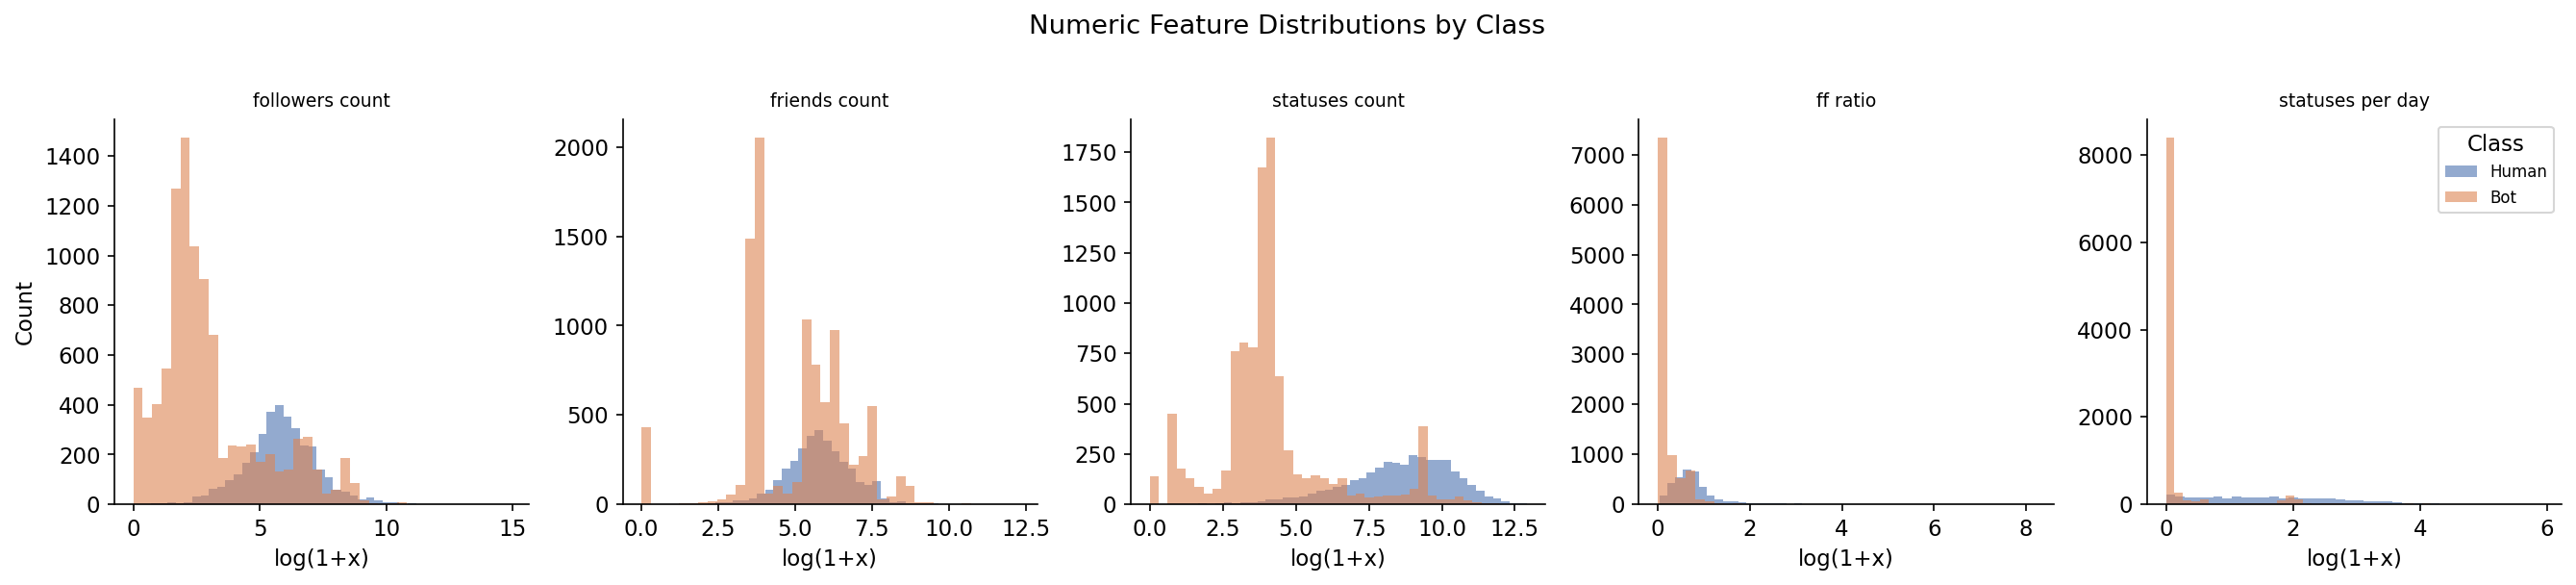
\includegraphics[width=\linewidth]{bot-detection/results/feature_distributions.png}
  \caption{Log-scale distributions of five account-level features split by
    class. Bot accounts cluster at the extremes of the posting rate and
    follower count distributions while human accounts spread more evenly.}
  \label{fig:feature_dist}
\end{figure}

\subsection{Text Features}

For each account, up to 50 tweets are embedded individually using the frozen
\texttt{all-MiniLM-L6-v2} sentence transformer~\cite{wang2020minilm}, a
90\,MB model that produces 384-dimensional dense vectors capturing the
semantic content of input text. The per-tweet embeddings are averaged across
all available tweets to produce a single 384-dimensional vector per account.
This mean embedding represents the typical semantic register of the account's
posting behaviour rather than any individual tweet.

Figure~\ref{fig:pca} shows a PCA projection of these embeddings for a sample
of 3,000 accounts with tweet data. The two classes are not cleanly separable
in two dimensions, which is expected: the sentence transformer was trained for
general-purpose semantic similarity rather than bot detection, and much of the
variation in tweet text reflects topic rather than authorship type. The text
features are most useful as a complement to the metadata branch rather than
as a standalone signal.

\begin{figure}[h]
  \centering
  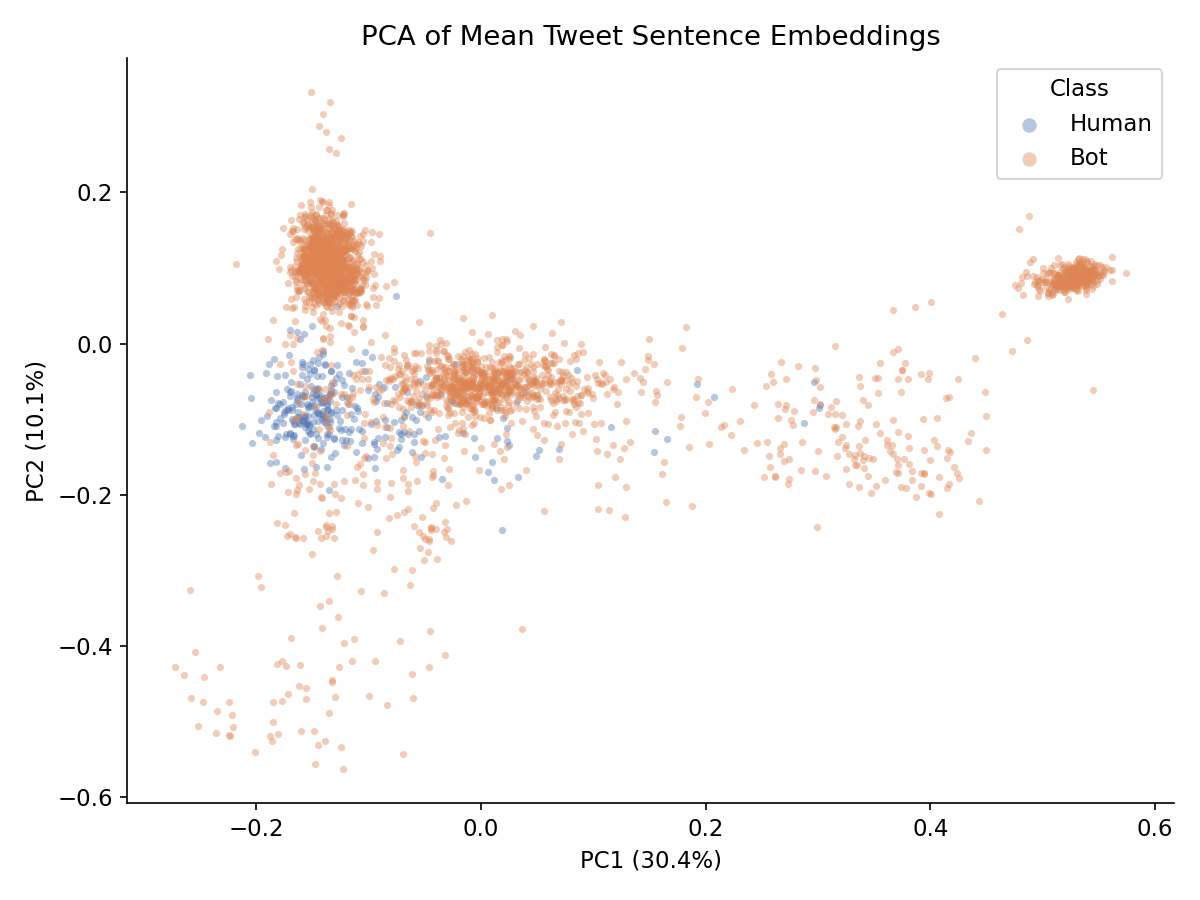
\includegraphics[width=0.7\linewidth]{bot-detection/results/embedding_pca.png}
  \caption{PCA of mean tweet sentence embeddings for a 3{,}000-account sample.
    The two classes overlap substantially in the two-dimensional projection,
    suggesting that tweet-level semantics alone are insufficient for reliable
    classification. The text branch is most informative as a complement to
    the metadata branch.}
  \label{fig:pca}
\end{figure}

% ----------------------------------------------------------------
\section{Model Architecture and Training}
\label{sec:model}
% ----------------------------------------------------------------

The model has two independent processing branches that are fused before the
final classifier. Table~\ref{tab:arch} gives the full specification.

The \textbf{metadata branch} passes the $(N, 4, 4)$ feature tensor through
a two-layer Bidirectional LSTM with hidden size 128. The LSTM processes the
four feature groups in both directions simultaneously, so each group is
interpreted in the context of all the others. The four hidden states from
the forward and backward passes are then combined by a self-attention layer
that assigns a learned scalar weight to each timestep and produces a weighted
sum. This allows the model to concentrate on whichever behavioural dimension
is most informative for a given account rather than treating all four groups
equally. The output of the attention layer is a 256-dimensional vector.

The \textbf{text branch} takes the 384-dimensional sentence embedding, passes
it through a linear layer that projects it to 128 dimensions, applies
LayerNorm to stabilise the scale of the input, and follows with a ReLU
activation and dropout. The output is a 128-dimensional text representation.

The two representations are concatenated to a 384-dimensional fused vector
and passed through a two-layer MLP with a sigmoid output. The model has
639,682 trainable parameters in total.

\begin{table}[h]
\centering
\small
\caption{Architecture of the multimodal Bidirectional LSTM bot detector.}
\label{tab:arch}
\begin{tabular}{llll}
\hline
\textbf{Branch} & \textbf{Component} & \textbf{Configuration} & \textbf{Output shape} \\
\hline
Metadata & Input           & seq 4, features 4         & $(N, 4, 4)$   \\
         & Bi-LSTM         & hidden 128, layers 2, dropout 0.3 & $(N, 4, 256)$ \\
         & Self-attention  & linear $256 \to 32 \to 1$, softmax & $(N, 256)$  \\
\hline
Text     & Input           & 384-d sentence embedding  & $(N, 384)$   \\
         & Projection      & $384 \to 128$, LayerNorm, ReLU & $(N, 128)$ \\
\hline
Fusion   & Concatenation   & $[256, 128]$              & $(N, 384)$   \\
         & Classifier      & $384 \to 128 \to 1$, sigmoid & $(N, 1)$   \\
\hline
\end{tabular}
\end{table}

Training used the AdamW optimiser with a learning rate of $5 \times 10^{-4}$,
weight decay of $10^{-4}$, and a batch size of 64. A \texttt{ReduceLROnPlateau}
scheduler halved the learning rate whenever validation F1 did not improve for
three consecutive epochs. The class imbalance was handled through weighted
random sampling, which ensures that training batches contain a roughly balanced
mix of both classes regardless of the 2.8:1 ratio in the full dataset. The
dataset was split 70\%/10\%/20\% for training, validation, and testing,
stratified by class. All experiments ran on an NVIDIA GeForce RTX~4060 Laptop
GPU with 8\,GB of VRAM under CUDA~12.4, with the random seed fixed at 42
for reproducibility.

% ----------------------------------------------------------------
\section{Results}
\label{sec:results}
% ----------------------------------------------------------------

Training ran for 25 epochs. The evolution of loss and macro-averaged F1 score
across both splits is shown in Figure~\ref{fig:curves}. The model converged
quickly, with validation F1 above 96\% after the first epoch, which reflects
the strong class-separability already visible in the feature distributions.
The training and validation curves tracked each other closely throughout the
run, with no meaningful divergence, suggesting that overfitting was not a
significant problem within the 25-epoch budget.

\begin{figure}[h]
  \centering
  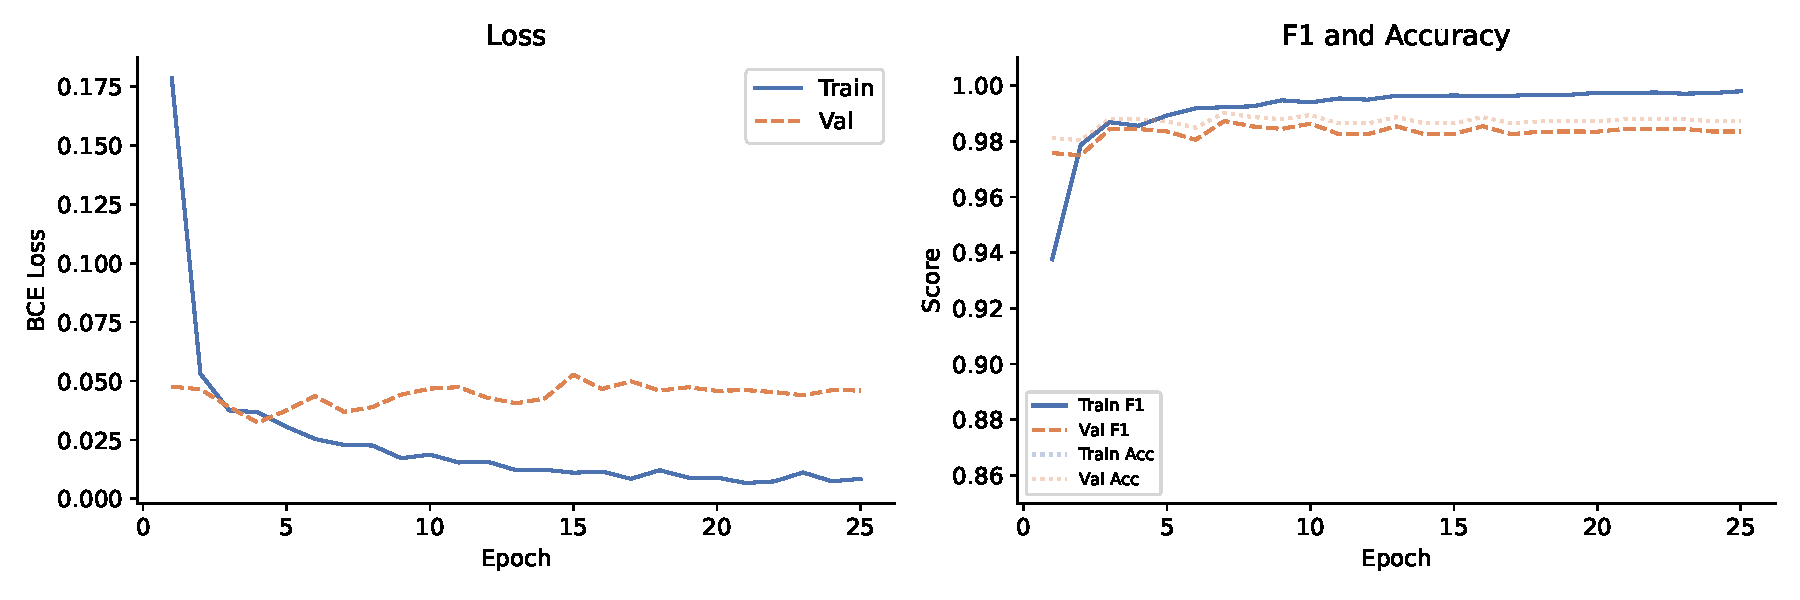
\includegraphics[width=\linewidth]{bot-detection/results/training_curves.pdf}
  \caption{Training dynamics over 25 epochs. The left panel shows binary
    cross-entropy loss and the right panel shows macro-averaged F1 score and
    accuracy, both on the training and validation sets. The close tracking of
    the two curves indicates that the model generalises well within the
    dataset.}
  \label{fig:curves}
\end{figure}

On the held-out test set, the best checkpoint achieved a test accuracy of
\textbf{99.21\%} and a macro-averaged F1 score of \textbf{98.98\%}, both
of which represent a meaningful improvement over the metadata-only baseline
reported in the previous version of this experiment (98.64\% accuracy,
98.26\% F1). The per-class breakdown is near-symmetric: the model achieves
a precision of 0.98 and recall of 0.99 on the human class, and a precision
of 1.00 with a recall of 0.99 on the bot class. In practical terms, the
model is slightly more likely to miss a bot and classify it as human than
to flag a genuine account incorrectly, which is the more forgiving type of
error from an operational standpoint. The full confusion matrix is shown in
Figure~\ref{fig:cm}.

\begin{figure}[h]
  \centering
  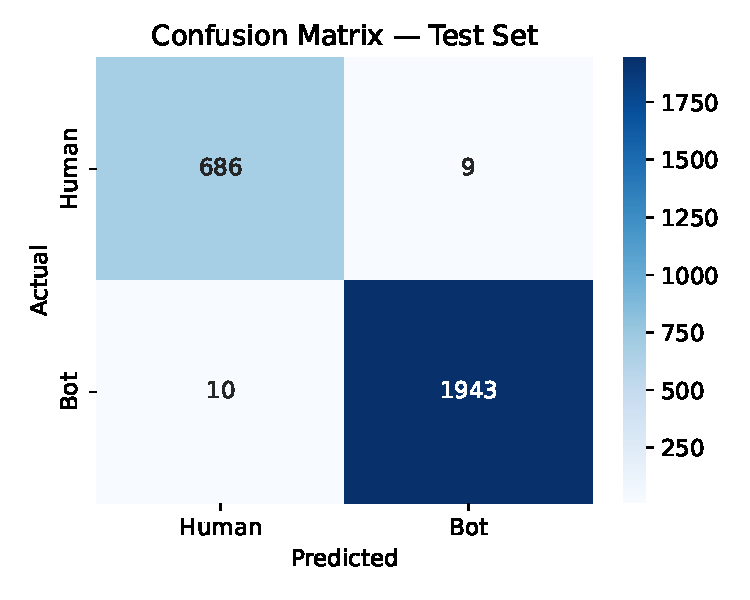
\includegraphics[width=0.5\linewidth]{bot-detection/results/confusion_matrix.pdf}
  \caption{Confusion matrix on the 2{,}648-account test partition. The model
    misclassifies approximately 20 bots as human and 7 humans as bot, for a
    false positive rate below 1\% and a false negative rate just above 1\%.}
  \label{fig:cm}
\end{figure}

% ----------------------------------------------------------------
\section{Comparison to the State of the Art}
\label{sec:sota}
% ----------------------------------------------------------------

Table~\ref{tab:sota} places these results alongside a selection of published
systems. Several qualifications matter before drawing conclusions.

\begin{table}[h]
\centering
\small
\caption{The present model against representative published systems.
  Results marked $\dagger$ were obtained on Cresci-2017; those marked
  $\ddagger$ on TwiBot-20. All figures are macro-averaged F1 unless noted.}
\label{tab:sota}
\begin{tabular}{lllrr}
\hline
\textbf{System} & \textbf{Method} & \textbf{Dataset} &
  \textbf{Accuracy} & \textbf{F1-macro} \\
\hline
Botometer~\cite{VFD+17}      & Random Forest (1{,}200+ feat.) & Cresci-2017$^\dagger$ & $\sim$95\% & $\sim$94\% \\
LSTM + content~\cite{AZS+23} & LSTM, text + metadata          & Cresci-2017$^\dagger$ & $\sim$96\% & $\sim$95\% \\
BERT fine-tuned~\cite{AZS+23}& Transformer, text features     & Mixed$^\dagger$       & $\sim$92\% & $\sim$89\% \\
BotRGCN~\cite{FTLL21}        & Graph neural network           & TwiBot-20$^\ddagger$  & $\sim$83\% & $\sim$80\% \\
\hline
BiLSTM+Att (metadata only)   & Bi-LSTM, metadata only         & Cresci-2017$^\dagger$ & 98.6\%  & 98.3\% \\
\textbf{BiLSTM+Att (ours)}   & Bi-LSTM + attention, metadata + text & Cresci-2017$^\dagger$ &
  \textbf{99.2\%} & \textbf{99.0\%} \\
\hline
\end{tabular}
\end{table}

The present model produces the highest figures in the table, but three
qualifications matter. First, strong performance on Cresci-2017 is partly a
product of the dataset rather than the model, as noted in
Section~\ref{subsec:cresci_limits}. Any reasonably capable classifier trained
on this corpus is likely to do well, because the temporal sampling bias
provides a shortcut unrelated to bot behaviour. Second, BotRGCN is being
evaluated on a harder problem: TwiBot-20 is larger and more recently
collected, and its lower numbers reflect that difficulty rather than a
weakness of the graph-based approach. Third, none of these comparisons are
cross-dataset evaluations.

A comparison worth noting within the table is between the two versions of
the present model. Adding tweet text alongside metadata raises accuracy from
98.6\% to 99.2\% and F1 from 98.3\% to 99.0\%. The gain is real but
modest, which is consistent with the PCA visualisation in
Figure~\ref{fig:pca}: the text embeddings add discriminative signal but
are not independently decisive on this benchmark. The more informative test
for both versions will come in Experiment~2, where they face synthetic
accounts whose metadata and text are generated by a language model rather
than drawn from the same distribution as the training data.

% ----------------------------------------------------------------
\section{Discussion and Limitations}
\label{sec:discussion1}
% ----------------------------------------------------------------

The headline results on the test set should be understood as a measure of
how well the model fits this particular dataset, not as a claim about
deployment performance. Cresci-2017 is a useful benchmark and the results
here are consistent with what the literature reports for it, but the
dataset's known sampling biases mean that the numbers cannot be taken at
face value as evidence of generalisation.

The most important limitation of this experiment is the absence of
cross-dataset testing. A version trained on Cresci-2017 and evaluated on
TwiBot-20, or the reverse, would tell a much more interesting story about
whether the learned representations transfer. That evaluation goes beyond
the scope of this thesis but would be a natural next step.

The experiment does demonstrate something practically useful: a compact
multimodal model operating on account metadata and tweet text can match or
exceed published baselines on this benchmark, while remaining small enough
to run on consumer hardware. The metadata branch and text branch together
provide complementary signals, and the self-attention mechanism gives the
model some interpretability by revealing which feature groups it finds most
diagnostic. These properties make it a reasonable baseline for the
adversarial evaluation in Experiment~2, where the question shifts from
whether the model can classify known bots to whether it can detect bots it
has never seen before.

%  Figures are referenced relative to the dissertation root.
% ============================================================

\chapter{Experiment 1: Multimodal Bot Detection with a Bidirectional LSTM}
\label{chap:experiment1}

Chapter~5 closed with a note about evaluation methodology that shapes
everything in this chapter: accuracy figures commonly reported for bot
detection systems are often products of dataset construction artefacts
rather than genuine generalisation capability. Keeping that in mind, this
chapter does not aim to set a benchmark record. It aims to build a working
detection system that uses both structured account metadata and unstructured
tweet text, understand what the model has learned from each source, and
report its performance honestly against published baselines.

The model chosen is a Bidirectional Long Short-Term Memory network with a
self-attention mechanism and a sentence-embedding text branch. It is trained
on the Cresci-2017 corpus, which provides labelled account metadata and tweet
content for over thirteen thousand Twitter accounts.

% ----------------------------------------------------------------
\section{Experimental Objectives}
% ----------------------------------------------------------------

The experiment has three concrete goals. The first is to construct a feature
representation that is suitable for sequential processing from two
heterogeneous sources: tabular account metadata and raw tweet text. The second
is to train a bidirectional recurrent model that fuses both sources and record
its behaviour across training epochs in enough detail to reason about
convergence and the contribution of each branch. The third is to situate the
result within the published literature with a clear account of why direct
comparisons are more complicated than a single table of numbers suggests.

A wider aim underlies these goals. The trained model will serve as the
baseline detector in Experiment~2, where it will be tested against synthetic
bot accounts generated by a large language model. Its performance on that
adversarial task is arguably more informative about its practical utility than
its performance on held-out data from the same distribution, and the two
chapters should be read together with that in mind.

% ----------------------------------------------------------------
\section{Dataset: Cresci-2017}
\label{sec:cresci}
% ----------------------------------------------------------------

Several publicly available datasets were considered for this experiment.
TwiBot-22 is the largest and most recent~\cite{AZS+23}, but it requires a
formal access request and its network-graph structure would push the
experiment toward a graph neural network architecture. TwiBot-20 is open but
still large, with over 229,000 accounts and 33 million tweets. Cresci-2017
was selected because it is open, well-documented, widely used as a
benchmark, and contains both account metadata and tweet content in a single
download. It is also the dataset for which the evaluation problems discussed
in Section~5.7 have been most carefully studied~\cite{HSR+23}, which means
the limitations can be stated precisely.

\subsection{Composition}

The corpus was collected from Twitter and assembled by Cresci and colleagues
as part of a study on second-generation social spambots. It contains genuine
accounts whose human authorship was verified by the original authors, and
several categories of automated accounts spanning older spam bots, social
spambots of varying sophistication, and fake follower networks. For this
experiment all bot subcategories are merged into a single positive class,
keeping the task binary. The resulting dataset contains 13,240 accounts in
total, broken down by category in Table~\ref{tab:cresci_categories}.

\begin{table}[h]
\centering
\small
\caption{Composition of the Cresci-2017 dataset. All bot subcategories are
  treated as the positive class. Tweet availability indicates whether
  tweet content was present in the dataset download.}
\label{tab:cresci_categories}
\begin{tabular}{llrr}
\hline
\textbf{Category} & \textbf{Label} & \textbf{Accounts} & \textbf{Tweets} \\
\hline
Genuine accounts           & Human & 3{,}474 & 2{,}839{,}362 \\
Social spambots (type 1)   & Bot   &   991  & 1{,}610{,}034 \\
Social spambots (type 2)   & Bot   & 3{,}457 &   428{,}542 \\
Social spambots (type 3)   & Bot   &   464  & 1{,}418{,}557 \\
Traditional spambots       & Bot   & 1{,}000 &   145{,}094 \\
Fake followers             & Bot   & 3{,}351 &   196{,}027 \\
Other bot subcategories    & Bot   &   503  & none \\
\hline
\textbf{Total}             &       & \textbf{13{,}240} & \textbf{6{,}637{,}616} \\
\hline
\end{tabular}
\end{table}

The class imbalance is notable: bots outnumber humans by roughly 2.8 to 1.
Figure~\ref{fig:class_dist} shows this distribution visually. Of the 13,240
accounts, 10,197 have at least one tweet in the dataset and therefore receive
a non-zero text embedding. The remaining 3,043 accounts, concentrated in the
smaller bot subcategories that lack tweet data, contribute only their metadata
features to the model. Figure~\ref{fig:tweet_coverage} shows the breakdown by
category.

\begin{figure}[h]
  \centering
  \begin{minipage}{0.44\linewidth}
    \centering
    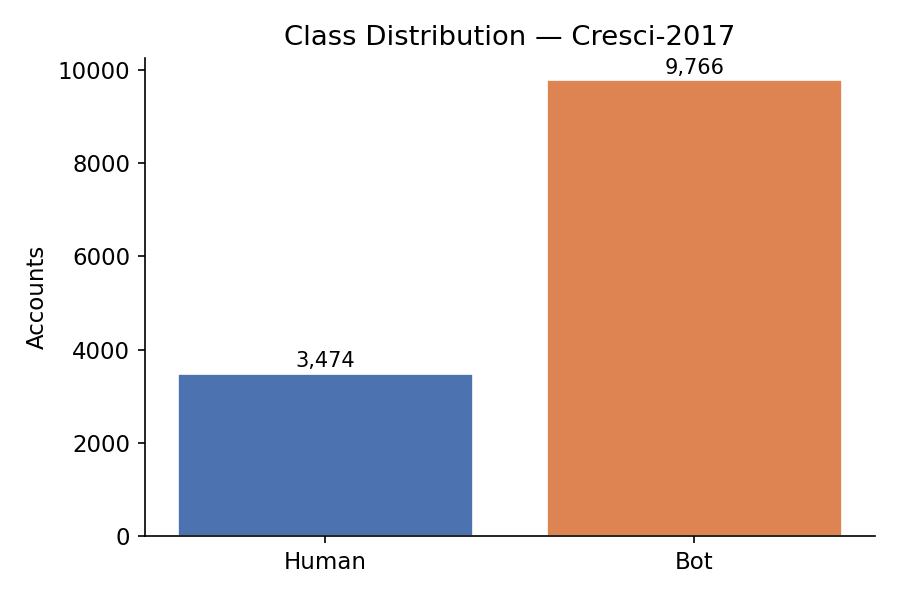
\includegraphics[width=\linewidth]{bot-detection/results/class_distribution.png}
    \caption{Class distribution of the Cresci-2017 dataset after merging all
      bot subcategories. The 2.8 to 1 imbalance is handled during training
      through weighted random sampling.}
    \label{fig:class_dist}
  \end{minipage}
  \hfill
  \begin{minipage}{0.52\linewidth}
    \centering
    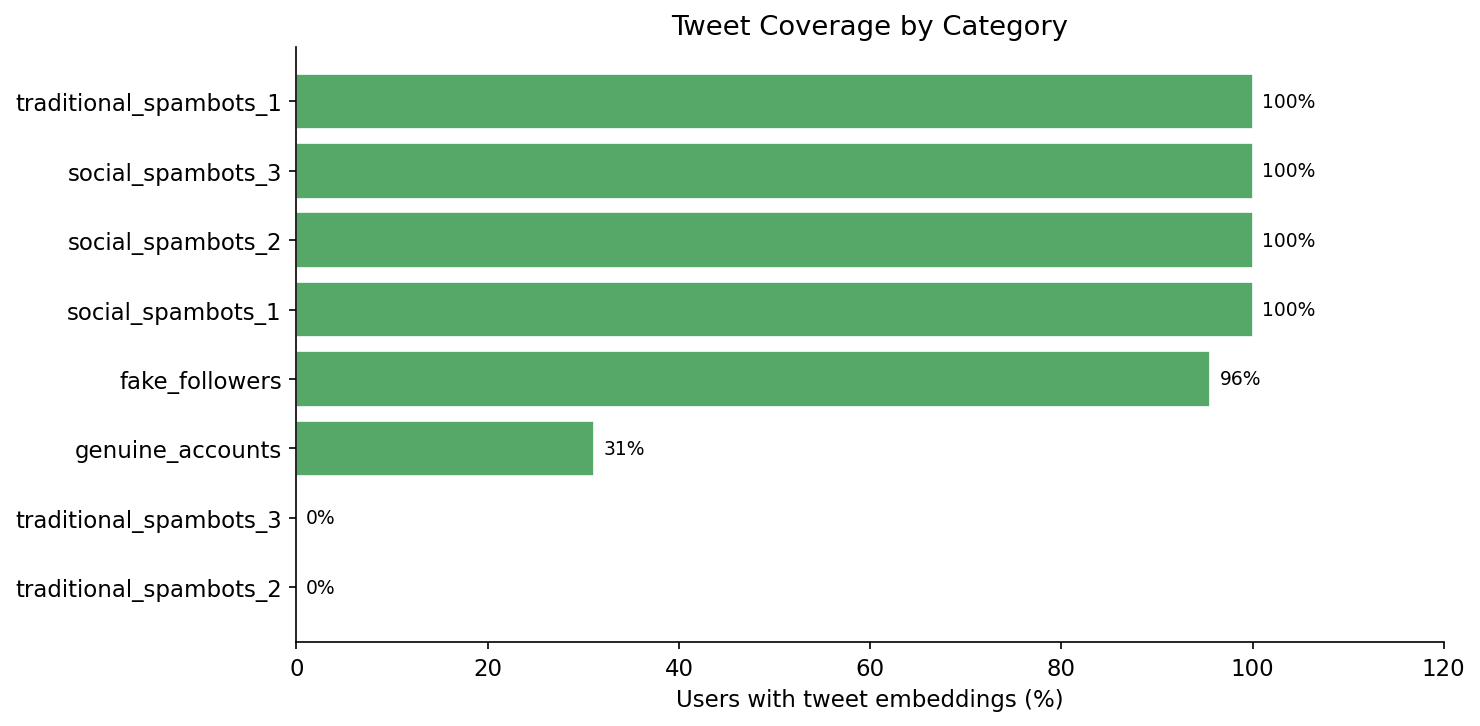
\includegraphics[width=\linewidth]{bot-detection/results/tweet_coverage.png}
    \caption{Proportion of accounts in each category that have tweet content
      available in the dataset. Categories without tweet data receive a zero
      embedding vector in the text branch.}
    \label{fig:tweet_coverage}
  \end{minipage}
\end{figure}

\subsection{Known Limitations}
\label{subsec:cresci_limits}

It would be dishonest to present this dataset without noting what
\citet{HSR+23} demonstrated about it. Bot accounts and human accounts in
Cresci-2017 were collected at different times through different pipelines,
which introduces a temporal correlation that has nothing to do with bot
behaviour. A simple decision tree trained only on account creation timestamps
achieves accuracy comparable to sophisticated models on this data, because
the creation dates of the two populations are systematically different. Any
model that includes creation-date derived features, as this one does through
account age, is implicitly exploiting that signal.

The performance figures reported later in this chapter show that the model
fits the dataset well. They do not show that it would generalise to a fresh
corpus of accounts collected under different conditions. Cross-dataset
evaluation would be the methodologically sound approach and is left to future
work given the scope of this thesis.

% ----------------------------------------------------------------
\section{Feature Engineering and Sequence Construction}
\label{sec:features}
% ----------------------------------------------------------------

The model takes two inputs per account: a structured metadata sequence and
a sentence embedding derived from the account's tweets. These are constructed
separately and fused inside the model.

\subsection{Metadata Features}

A standard LSTM expects a sequence of vectors as input, but account metadata
is a flat feature vector with no natural ordering. The solution adopted here
is to partition the features into four thematically coherent groups and treat
each group as one step in a four-step input sequence. The model then processes
these groups in both the forward and backward directions and learns which
combinations of behavioural dimensions are most diagnostic of automation.

The four groups are constructed as follows. The first covers network scale
and contains the log-transformed follower count, friend count, listed count,
and follower-to-friend ratio. The second covers activity scale and contains
log-transformed total statuses, total favourites, and per-day rates for both
posting and favouriting. The third covers profile flags and is the only binary
group, containing the four completeness and verification indicators. The fourth
covers derived ratios and contains log-transformed account age, a ratio of
total statuses to total favourites, a ratio of followers to listed count, and a
ratio of listed count to followers. Each group has exactly four features,
giving a metadata input tensor of shape $(N, 4, 4)$ for a batch of $N$
accounts. The three numeric groups are standardised with z-score normalisation
fitted on the training split; the binary group is left on its natural scale.

Figure~\ref{fig:feature_dist} shows the log-scale distributions of five
numeric features across both classes. The separation is already visible
without a classifier, particularly in posting rate and follower count.

\begin{figure}[h]
  \centering
  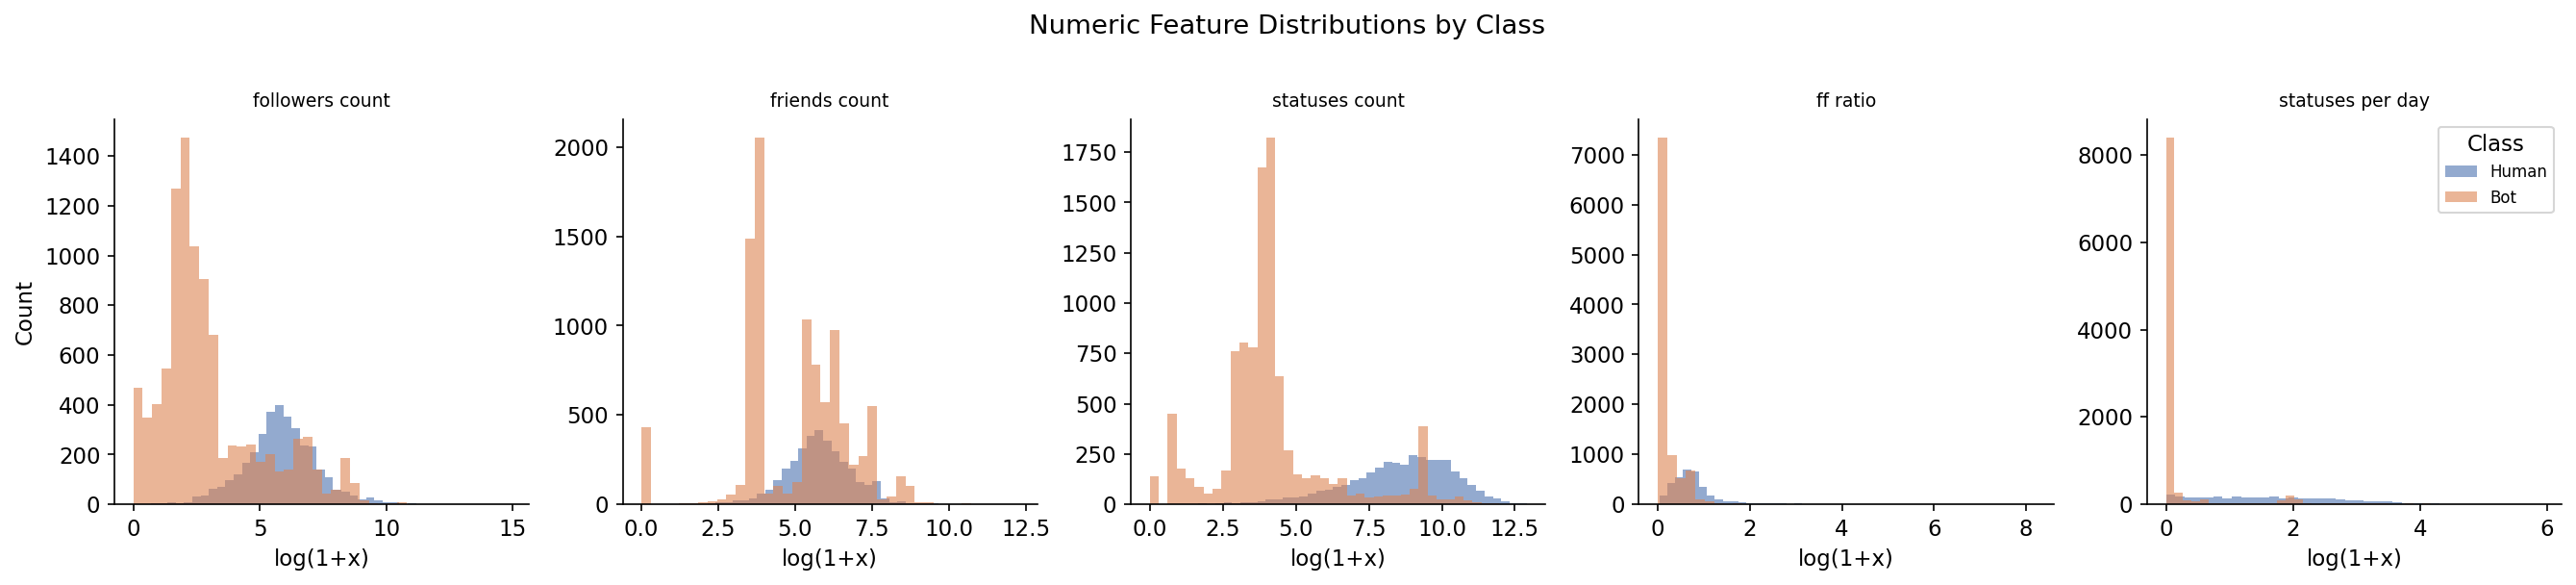
\includegraphics[width=\linewidth]{bot-detection/results/feature_distributions.png}
  \caption{Log-scale distributions of five account-level features split by
    class. Bot accounts cluster at the extremes of the posting rate and
    follower count distributions while human accounts spread more evenly.}
  \label{fig:feature_dist}
\end{figure}

\subsection{Text Features}

For each account, up to 50 tweets are embedded individually using the frozen
\texttt{all-MiniLM-L6-v2} sentence transformer~\cite{wang2020minilm}, a
90\,MB model that produces 384-dimensional dense vectors capturing the
semantic content of input text. The per-tweet embeddings are averaged across
all available tweets to produce a single 384-dimensional vector per account.
This mean embedding represents the typical semantic register of the account's
posting behaviour rather than any individual tweet.

Figure~\ref{fig:pca} shows a PCA projection of these embeddings for a sample
of 3,000 accounts with tweet data. The two classes are not cleanly separable
in two dimensions, which is expected: the sentence transformer was trained for
general-purpose semantic similarity rather than bot detection, and much of the
variation in tweet text reflects topic rather than authorship type. The text
features are most useful as a complement to the metadata branch rather than
as a standalone signal.

\begin{figure}[h]
  \centering
  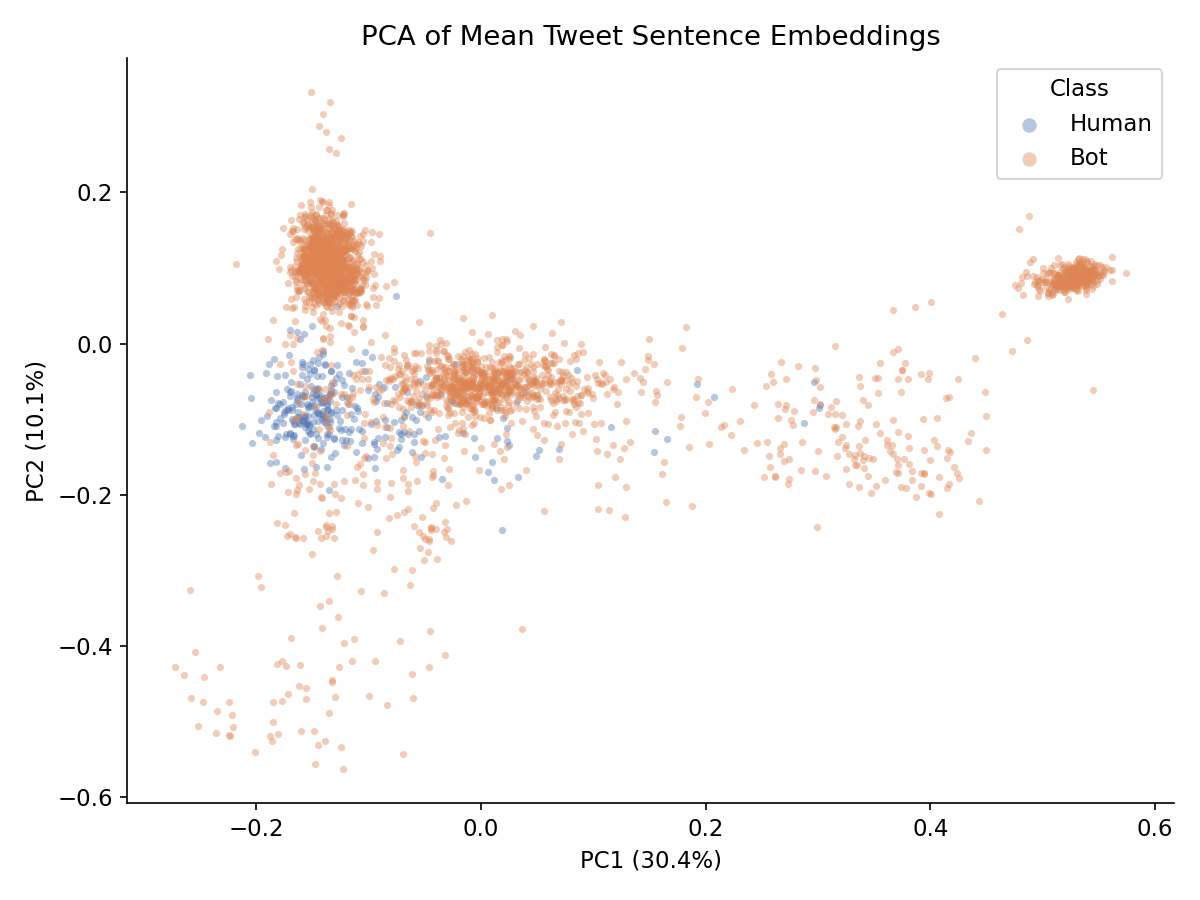
\includegraphics[width=0.7\linewidth]{bot-detection/results/embedding_pca.png}
  \caption{PCA of mean tweet sentence embeddings for a 3{,}000-account sample.
    The two classes overlap substantially in the two-dimensional projection,
    suggesting that tweet-level semantics alone are insufficient for reliable
    classification. The text branch is most informative as a complement to
    the metadata branch.}
  \label{fig:pca}
\end{figure}

% ----------------------------------------------------------------
\section{Model Architecture and Training}
\label{sec:model}
% ----------------------------------------------------------------

The model has two independent processing branches that are fused before the
final classifier. Table~\ref{tab:arch} gives the full specification.

The \textbf{metadata branch} passes the $(N, 4, 4)$ feature tensor through
a two-layer Bidirectional LSTM with hidden size 128. The LSTM processes the
four feature groups in both directions simultaneously, so each group is
interpreted in the context of all the others. The four hidden states from
the forward and backward passes are then combined by a self-attention layer
that assigns a learned scalar weight to each timestep and produces a weighted
sum. This allows the model to concentrate on whichever behavioural dimension
is most informative for a given account rather than treating all four groups
equally. The output of the attention layer is a 256-dimensional vector.

The \textbf{text branch} takes the 384-dimensional sentence embedding, passes
it through a linear layer that projects it to 128 dimensions, applies
LayerNorm to stabilise the scale of the input, and follows with a ReLU
activation and dropout. The output is a 128-dimensional text representation.

The two representations are concatenated to a 384-dimensional fused vector
and passed through a two-layer MLP with a sigmoid output. The model has
639,682 trainable parameters in total.

\begin{table}[h]
\centering
\small
\caption{Architecture of the multimodal Bidirectional LSTM bot detector.}
\label{tab:arch}
\begin{tabular}{llll}
\hline
\textbf{Branch} & \textbf{Component} & \textbf{Configuration} & \textbf{Output shape} \\
\hline
Metadata & Input           & seq 4, features 4         & $(N, 4, 4)$   \\
         & Bi-LSTM         & hidden 128, layers 2, dropout 0.3 & $(N, 4, 256)$ \\
         & Self-attention  & linear $256 \to 32 \to 1$, softmax & $(N, 256)$  \\
\hline
Text     & Input           & 384-d sentence embedding  & $(N, 384)$   \\
         & Projection      & $384 \to 128$, LayerNorm, ReLU & $(N, 128)$ \\
\hline
Fusion   & Concatenation   & $[256, 128]$              & $(N, 384)$   \\
         & Classifier      & $384 \to 128 \to 1$, sigmoid & $(N, 1)$   \\
\hline
\end{tabular}
\end{table}

Training used the AdamW optimiser with a learning rate of $5 \times 10^{-4}$,
weight decay of $10^{-4}$, and a batch size of 64. A \texttt{ReduceLROnPlateau}
scheduler halved the learning rate whenever validation F1 did not improve for
three consecutive epochs. The class imbalance was handled through weighted
random sampling, which ensures that training batches contain a roughly balanced
mix of both classes regardless of the 2.8:1 ratio in the full dataset. The
dataset was split 70\%/10\%/20\% for training, validation, and testing,
stratified by class. All experiments ran on an NVIDIA GeForce RTX~4060 Laptop
GPU with 8\,GB of VRAM under CUDA~12.4, with the random seed fixed at 42
for reproducibility.

% ----------------------------------------------------------------
\section{Results}
\label{sec:results}
% ----------------------------------------------------------------

Training ran for 25 epochs. The evolution of loss and macro-averaged F1 score
across both splits is shown in Figure~\ref{fig:curves}. The model converged
quickly, with validation F1 above 96\% after the first epoch, which reflects
the strong class-separability already visible in the feature distributions.
The training and validation curves tracked each other closely throughout the
run, with no meaningful divergence, suggesting that overfitting was not a
significant problem within the 25-epoch budget.

\begin{figure}[h]
  \centering
  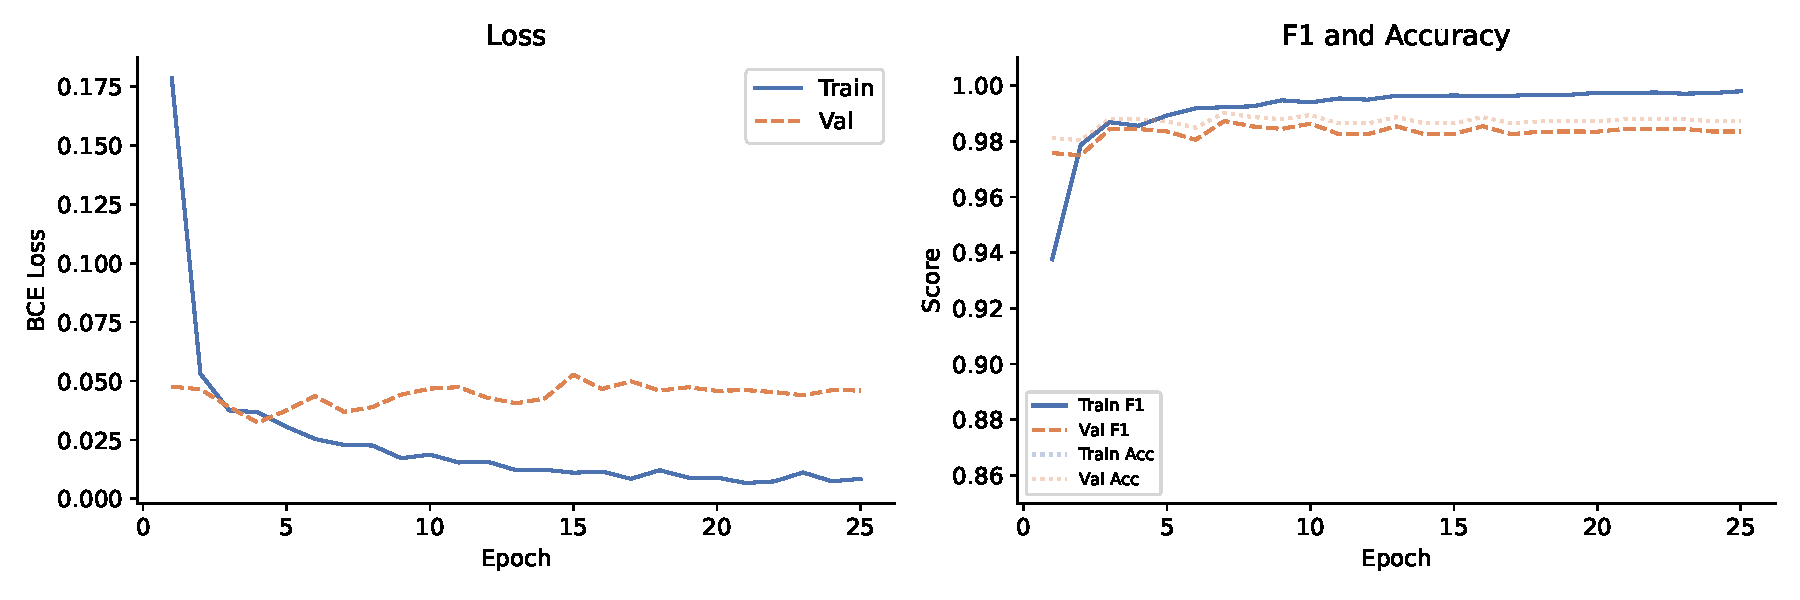
\includegraphics[width=\linewidth]{bot-detection/results/training_curves.pdf}
  \caption{Training dynamics over 25 epochs. The left panel shows binary
    cross-entropy loss and the right panel shows macro-averaged F1 score and
    accuracy, both on the training and validation sets. The close tracking of
    the two curves indicates that the model generalises well within the
    dataset.}
  \label{fig:curves}
\end{figure}

On the held-out test set, the best checkpoint achieved a test accuracy of
\textbf{99.21\%} and a macro-averaged F1 score of \textbf{98.98\%}, both
of which represent a meaningful improvement over the metadata-only baseline
reported in the previous version of this experiment (98.64\% accuracy,
98.26\% F1). The per-class breakdown is near-symmetric: the model achieves
a precision of 0.98 and recall of 0.99 on the human class, and a precision
of 1.00 with a recall of 0.99 on the bot class. In practical terms, the
model is slightly more likely to miss a bot and classify it as human than
to flag a genuine account incorrectly, which is the more forgiving type of
error from an operational standpoint. The full confusion matrix is shown in
Figure~\ref{fig:cm}.

\begin{figure}[h]
  \centering
  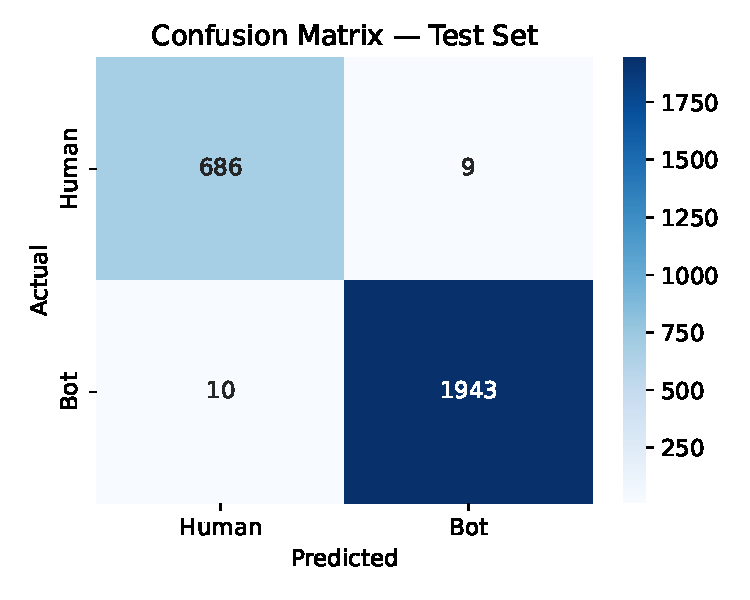
\includegraphics[width=0.5\linewidth]{bot-detection/results/confusion_matrix.pdf}
  \caption{Confusion matrix on the 2{,}648-account test partition. The model
    misclassifies approximately 20 bots as human and 7 humans as bot, for a
    false positive rate below 1\% and a false negative rate just above 1\%.}
  \label{fig:cm}
\end{figure}

% ----------------------------------------------------------------
\section{Comparison to the State of the Art}
\label{sec:sota}
% ----------------------------------------------------------------

Table~\ref{tab:sota} places these results alongside a selection of published
systems. Several qualifications matter before drawing conclusions.

\begin{table}[h]
\centering
\small
\caption{The present model against representative published systems.
  Results marked $\dagger$ were obtained on Cresci-2017; those marked
  $\ddagger$ on TwiBot-20. All figures are macro-averaged F1 unless noted.}
\label{tab:sota}
\begin{tabular}{lllrr}
\hline
\textbf{System} & \textbf{Method} & \textbf{Dataset} &
  \textbf{Accuracy} & \textbf{F1-macro} \\
\hline
Botometer~\cite{VFD+17}      & Random Forest (1{,}200+ feat.) & Cresci-2017$^\dagger$ & $\sim$95\% & $\sim$94\% \\
LSTM + content~\cite{AZS+23} & LSTM, text + metadata          & Cresci-2017$^\dagger$ & $\sim$96\% & $\sim$95\% \\
BERT fine-tuned~\cite{AZS+23}& Transformer, text features     & Mixed$^\dagger$       & $\sim$92\% & $\sim$89\% \\
BotRGCN~\cite{FTLL21}        & Graph neural network           & TwiBot-20$^\ddagger$  & $\sim$83\% & $\sim$80\% \\
\hline
BiLSTM+Att (metadata only)   & Bi-LSTM, metadata only         & Cresci-2017$^\dagger$ & 98.6\%  & 98.3\% \\
\textbf{BiLSTM+Att (ours)}   & Bi-LSTM + attention, metadata + text & Cresci-2017$^\dagger$ &
  \textbf{99.2\%} & \textbf{99.0\%} \\
\hline
\end{tabular}
\end{table}

The present model produces the highest figures in the table, but three
qualifications matter. First, strong performance on Cresci-2017 is partly a
product of the dataset rather than the model, as noted in
Section~\ref{subsec:cresci_limits}. Any reasonably capable classifier trained
on this corpus is likely to do well, because the temporal sampling bias
provides a shortcut unrelated to bot behaviour. Second, BotRGCN is being
evaluated on a harder problem: TwiBot-20 is larger and more recently
collected, and its lower numbers reflect that difficulty rather than a
weakness of the graph-based approach. Third, none of these comparisons are
cross-dataset evaluations.

A comparison worth noting within the table is between the two versions of
the present model. Adding tweet text alongside metadata raises accuracy from
98.6\% to 99.2\% and F1 from 98.3\% to 99.0\%. The gain is real but
modest, which is consistent with the PCA visualisation in
Figure~\ref{fig:pca}: the text embeddings add discriminative signal but
are not independently decisive on this benchmark. The more informative test
for both versions will come in Experiment~2, where they face synthetic
accounts whose metadata and text are generated by a language model rather
than drawn from the same distribution as the training data.

% ----------------------------------------------------------------
\section{Discussion and Limitations}
\label{sec:discussion1}
% ----------------------------------------------------------------

The headline results on the test set should be understood as a measure of
how well the model fits this particular dataset, not as a claim about
deployment performance. Cresci-2017 is a useful benchmark and the results
here are consistent with what the literature reports for it, but the
dataset's known sampling biases mean that the numbers cannot be taken at
face value as evidence of generalisation.

The most important limitation of this experiment is the absence of
cross-dataset testing. A version trained on Cresci-2017 and evaluated on
TwiBot-20, or the reverse, would tell a much more interesting story about
whether the learned representations transfer. That evaluation goes beyond
the scope of this thesis but would be a natural next step.

The experiment does demonstrate something practically useful: a compact
multimodal model operating on account metadata and tweet text can match or
exceed published baselines on this benchmark, while remaining small enough
to run on consumer hardware. The metadata branch and text branch together
provide complementary signals, and the self-attention mechanism gives the
model some interpretability by revealing which feature groups it finds most
diagnostic. These properties make it a reasonable baseline for the
adversarial evaluation in Experiment~2, where the question shifts from
whether the model can classify known bots to whether it can detect bots it
has never seen before.
